% !TEX program = xelatex
% !TeX encoding = utf8
% !TeX spellcheck = pl-PL

%%%%%%%%%%%%%%%%%%%%%%%%%%%%%%%%%%%%%%%%%%%%%%%%%%%%%%%%%%%%%%%%%%%%%%%%%%%
% Wybierz rodzaj pracy dyplomowej oraz wydział
% Pick thesis type and faculty
%%%%%%%%%%%%%%%%%%%%%%%%%%%%%%%%%%%%%%%%%%%%%%%%%%%%%%%%%%%%%%%%%%%%%%%%%%%
\documentclass[thesis=inz,faculty=ee]{EE-dyplom} 
\usepackage{mathspec,amssymb,bbm,graphicx}
% unicode-math,
\usepackage{csquotes} %% <- added !
%\usepackage{mathspec, amssymb, bbm} % , graphicx
%\setmathfont{Latin Modern Math} 
%\usepackage{parskip} %% <- added !
% thesis=[inz|mgr|bsc|msc]
%  * inz - praca inżynierska
%  * mgr - praca magisterska
%  * bsc - bachelor thesis
%  * msc - master thesis
% Skróty nazw wydziałów zgodne z domenami internetowymi
% Abbreviations of Faculties according to Internet subdomains
% faculty=[
%	arch,
%	gik,
%	ee,
%	wip
%	]

%%%%%%%%%%%%%%%%%%%%%%%%%%%%%%%%%%%%%%%%%%%%%%%%%%%%%%%%%%%%%%%%%%%%%%%%%%%
% Konfiguracja - do personalizacji
% Configuration - to be personalized
%%%%%%%%%%%%%%%%%%%%%%%%%%%%%%%%%%%%%%%%%%%%%%%%%%%%%%%%%%%%%%%%%%%%%%%%%%%
\instytut{Instytut Sterowania i Elektroniki Przemysłowej}
\kierunek{Informatyka Stosowana}
\specjalnosc{Informatyka Stosowana}
\title{Porównanie wydajności wybranych języków programowania w realizacji sieci neuronowych do przetwarzania obrazów}
\engtitle{Comparison of the performance of selected programming languages in the implementation of neural networks for image processing}
\album{146703}
\author{Piotr Heinzelman}
\promotor{dr inż. Witold Czajewski}
\date{2025}
\longdate{2025-06-20}

%\grantlicense{TRUE} % [TRUE|FALSE]

%%%%%%%%%%%%%%%%%%%%%%%%%%%%%%%%%%%%%%%%%%%%%%%%%%%%%%%%%%%%%%%%%%%%%%%%%%%
% Streszczenie pracy i abstract.
% In case of thesis in English swap the order - English version goes first.
%%%%%%%%%%%%%%%%%%%%%%%%%%%%%%%%%%%%%%%%%%%%%%%%%%%%%%%%%%%%%%%%%%%%%%%%%%%
\streszczeniepracy{ 
W niniejszej pracy poruszono zagadnienia tworzenia wysokowydajnych systemów obliczeniowych w~celu realizacji modeli głębokich sieci neuronowych. Duże modele wymagają efektywnych sposobów obliczania odpowiedzi sieci i prowadzenia procesu uczenia, ponieważ wraz ze wzrostem wielkości modelu wyraźnie wzrasta czas wykonywania obliczeń.

Przypomniano sposoby zwiększania wydajności sprzętu, zwłaszcza te, które mogą być zastosowane w modelach sieci neuronowych.

We wprowadzeniu przybliżono matematyczne modele sieci CNN i MLP, a następnie rozpisano realizację tych modeli jako sekwencję działań arytmetycznych. Zwrócono uwagę na możliwość zwiększenia wydajności poprzez realizację przetwarzania w sposób równoległy.

Zaprezentowano pokrótce zadania postawione do wykonania porównywanym modelom.

W pracy dokonano porównania takich własności języków jak: popularność, dostępność bibliotek, wygoda instalacji, wsparcie obliczeń na kartach graficznych, stopień trudności języka, koszt licencji. Zaprezentowano również fragmenty kodu, a także opisano doświadczenia w trakcie pisania kodu. 

Omówiono wybrane języki: Python, Maltab, Java, C++. Do budowania sieci Yolo8 wykorzystano biblioteki: Torch, Ultralytics. W projektach sieci CNN użyto: TensorFlow, Scikit-Learn, PyTorch. W projektach Matlab użyto pakietu Deep Learning Toolbox. W języju Java wykorzystano własne implementacje.


W podsumowaniu zebrano wyniki, oraz zaprezentowano przesłanki, które mogą być pomocne przy doborze języka w celu realizacji głębokich sieci neuronowych.
} % koniec streszczenia

\slowakluczowe{uczenie głębokich sieci neuronowych, sieci splotowe CNN, YOLO, wydajność, klasyfikacja obrazów, obliczenia równoległe, dodawanie sekwencyjne}

\thesisabstract{
This paper addresses the issues of creating high-performance computing systems to implement deep neural network models. Large models require effective methods of calculating network responses and conducting the learning process, because the larger the model size, the more computational time is needed.

Methods of increasing hardware performance are recalled, especially those that can be used in neural network models.

The introduction presents mathematical models of CNN and MLP networks, and then describes the implementation of these models as a sequence of arithmetic operations. Attention is drawn to the possibility of increasing performance by implementing parallel processing.

The tasks set for the compared models are briefly presented.

The paper compares such language properties as: popularity, availability of libraries, ease of installation, support for computing on graphics cards, language difficulty level, and license cost. Code fragments are also presented, and experiences during writing the code are described.

Selected languages are discussed: Python, Maltab, Java, C++. The following libraries were used to build the Yolo8 network: Torch, Ultralytics. In the CNN projects, the following were used: TensorFlow, Scikit-Learn, PyTorch. In the Matlab projects, the Deep Learning Toolbox was used. In Java, own implementations were used.

The summary summarizes the results and presents premises that may be helpful in selecting a language for implementing deep neural networks.

} % end of abstract

\thesiskeywords{deep learning, convolution network, image clasification, efficiency, parallel computing }

%%%%%%%%%%%%%%%%%%%%%%%%%%%%%%%%%%%%%%%%%%%%%%%%%%%%%%%%%%%%%%%%%%%%%%%%%%%
% Tu zaczyna się dokument
% Here is the beginning of the document
%%%%%%%%%%%%%%%%%%%%%%%%%%%%%%%%%%%%%%%%%%%%%%%%%%%%%%%%%%%%%%%%%%%%%%%%%%%
\begin{document}
    % Strony nagłówkowe - musi być
    % Headers - must exist
    \frontpages
    
    % Tekst pracy - osobne pliki do edycji
    % Thesis text - separate files for edition

% *****************************    

%\chapter{Wstęp}
%Dobór algorytmu do zadania jest bardzo ważny, zdecydowanie ważniejszy niż dobór języka - jednak nie będzie on głównym tematem tej pracy. Tu zakładamy użycie tych samych algorytmów i porównujemy wydajności implementacji algorytmu w różnych "językach". Teoretycznie wyniki powinny być zbliżone przy założeniu, że programy doskonale wykorzystują możliwości sprzętu. Celem pracy jest porównanie, które języki ogólnego przeznaczenia liczą szybciej, które lepiej wykorzystują dodatkową infrastrukturę taką jak \textit{wątki}, \textit{procesy},  \textit{hyperThreading}, czy rdzenie \textit{CUDA} na kartach graficznych.
Jeśli gdzieś zaobserwujemy różnice - to będą one wynikały zastosowania innych języków, które w odmienny sposób zapisują i odczytują liczby, kolejkują zadania czy optymalizują wygenerowany kod. \newLine 
Jednak zanim przejdziemy do~porównania, przyjrzymy się modelom matematycznym, a z ich pomocą zbudujemy prosty model obiektowy. Następnie przetestujemy model obiektowy, prześledzimy przetwarzanie na najniższych poziomach, aż do pojedynczych operacji. Te działania pomogą nam przygotować zadania numeryczne, do rozwiązania których użyjemy maszyn cyfrowych.

\begin{lstlisting}
/*

4. Realizacje obliczeń Klasyfikowanie pisma odręcznego MLP z wykorzystaniem danych MNIST
a) Matlab
b) Python -numpy, -sklearn
c) Python -tensorflow
d) własna implementacja w Java

Cel podstawowy: porównanie wydajności realizacji w zależności od Języka.
Cele dodatkowe: potwierdzenie poprawności własnej implementacji przez porównanie wyników,


5) realizacja Klasyfikowanie pisma odręcznego sieci głębokie CNN realizacja sieci z wykorzytsniem bibliotek.
a) Matlab
b) Python tensorflow.keras
c) własna implementacja Java lub C++ libtorch

Cel podstawowy: porównanie wydajności implementacji. Zbadanie wydajności uczenia sieci.
Cele dodatkowe: potwierdzenie poprawności własnej implementacji w Java lub C++


6) Rozpoznawanie twarzy sieci głębokie CNN
a) Matlab
b) Python tensorflow.keras
c) własna implementacja Java lub C++ libtorch

Cel podstawowy: porównanie wydajności implementacji.


7) Klasyfikacji obrazów z wykorzystaniem sieci głębokiej CNN
a) Matlab
b) Python tensorflow.keras
c) C++ libtorch

Cel podstawowy: porównanie wydajności implementacji i wydajności procesu uczenia nadzorowanego.

8) detekcja i segmentacji obiektów sieci głębokiej CNN
b) Python tensorflow.keras
c) C++ libtorch

Cel podstawowy: porównanie wydajności implementacji.


*/
\end{lstlisting}

    %\chapter{Yolo}
    %% \section{ Układ pracy }
% W pierwszej części opisano proces przygotowania i uruchamiania sieci Yolo w różnych środowiskach, opisano aspekty takie jak wygoda tworzenia rozwiązania, dostęp do dokumentacji, ilość dostępnych przykładów.

% Yolo Matlab v3
% https://www.mathworks.com/help/vision/ref/yolov3objectdetector.html
% autorun Example: openExample('vision/DetectObjectsUsingYOLOV3DetectorExample')

% Yolo Matlab v4
% https://www.mathworks.com/help/vision/ug/getting-started-with-yolo-v4.html


% OPEN !! 
% https://viso.ai/deep-learning/yolov3-overview/


 

%%%
%%% C++
%%%
% https://medium.com/@siromermer/running-yolo-models-in-c-for-object-detection-a698b3b7cd5f
% https://github.com/ultralytics/ultralytics/tree/main/examples/YOLOv8-LibTorch-CPP-Inference
% !!!
% https://github.com/ultralytics/ultralytics/tree/main/docs/en/datasets/detect 
%%%
% https://github.com/ultralytics/ultralytics/issues/1852

% https://www.reddit.com/r/opencv/comments/144m4tt/tutorials_yolov8_with_opencv_and_tensorrt_c_link/
% https://github.com/cyrusbehr/YOLOv8-TensorRT-CPP
% https://community.ultralytics.com/t/cpp-inference-of-yolov8/85
% https://medium.com/@siromermer/running-yolo-models-in-c-for-object-detection-a698b3b7cd5f
% https://docs.ultralytics.com/
% https://yolov8.com/
% https://github.com/Geekgineer/YOLOs-CPP
% !!!!!!!!!!!!
% https://github.com/ultralytics/ultralytics/issues/671
% https://learnopencv.com/object-detection-using-yolov5-and-opencv-dnn-in-c-and-python/



YOLO (You Only Look Once), popularny model do wykrywania obiektów i segmentacji obrazu, został opracowany przez Josepha Redmona i Alego Farhadiego na Uniwersytecie Waszyngtońskim. Wprowadzony na rynek w 2015 roku, YOLO zyskał popularność dzięki wysokiej szybkości i dokładności.
Odpowiedni model Yolo można pobrać w wersji wytrenowanej i dotrenować do własnych danych co jest rozwiązaniem szybszym i łatwiejszym do przeprowadzenia lub trenować tylko na własnych danych. W modelach Yolo trenowane są osobno bloki warstw odpowiadające za klasyfikację obiektów, a osobno warstwy odpowiadające za segmentacje. Skutek ten osiąga się przez "zamrożenie" warstw.

Modele Yolo we wszystkich wersjach mają podobną budowę i złożone są z bloków warstw:
\begin{itemize}
    \item blok wejściowy składa się z warstw splotowych CNN ;
    \item blok wyjściowy klasyfikacji składa się z warstw FC / MLP;
    \item blok segmentacji składa się z warstw FC, w nowszych rozwiązaniach także z warstw splotowych;
\end{itemize}

Kolejne wydania różnią się sposobem przekazywania sygnałów między blokami.
Większość obliczeń wykonywanych jest w warstwach CNN i MLP, z tego powodu mają największy wpływ czas trwania procesów predykcji i uczenia. Dlatego wpływ opóźnień powstający w tych warstwach ma wpływ na czas predykcji, testowania i uczenia modeli, i z tego powodu właśnie te dwie warstwy zostaną przebadane i opisane dokładnie w następnych częściach niniejszej pracy.

\section{Yolo}
\begin{itemize}
    \item YOLO, 
    \item YOLOv2, wydany w 2016 roku, ulepszył oryginalny model, wprowadzając normalizację wsadową, pola kotwiczące i klastry wymiarów \cite{redmon2016yolo9000betterfasterstronger}.
    \item YOLOv3, wydany w 2018 roku, dodatkowo poprawił wydajność modelu, wykorzystując wydajniejszą sieć szkieletową, wiele kotwic i łączenie piramid przestrzennych.
    \item YOLOv4, wydany w 2020 roku, wprowadził innowacje, takie jak rozszerzenie danych Mosaic, nową głowicę detekcyjną bez kotwic i nową funkcję strat.
    \item YOLOv5 dodatkowo poprawił wydajność modelu i dodał nowe funkcje, takie jak optymalizacja hiperparametrów, zintegrowane śledzenie eksperymentów i automatyczny eksport do popularnych formatów eksportu.
    \item YOLOv6 został udostępniony jako oprogramowanie open source przez Meituan w 2022 roku i jest wykorzystywany w wielu autonomicznych robotach dostawczych tej firmy.
    \item YOLOv7 dodał dodatkowe zadania, takie jak szacowanie pozycji w zbiorze danych punktów kluczowych COCO.
    \item YOLOv8, wydany w 2023 roku przez Ultralytics, wprowadził nowe funkcje i ulepszenia zwiększające wydajność, elastyczność i efektywność, obsługując pełen zakres zadań sztucznej inteligencji wizyjnej.
    \item YOLOv9 wprowadza innowacyjne metody, takie jak programowalna informacja gradientowa (PGI) i uogólniona efektywna sieć agregacji warstw (GELAN).
    \item YOLOv10, stworzony przez naukowców z Uniwersytetu Tsinghua z wykorzystaniem pakietu Ultralytics Python, zapewnia udoskonalenia w zakresie wykrywania obiektów w czasie rzeczywistym dzięki wprowadzeniu głowicy End-to-End, która eliminuje wymagania dotyczące tłumienia niemaksymalnego (NMS).
    \item YOLO11 Najnowsze modele YOLO firmy Ultralytics zapewniają najwyższą wydajność (SOTA) w wielu zadaniach, w tym wykrywaniu obiektów, segmentacji, szacowaniu pozycji, śledzeniu i klasyfikacji, wykorzystując możliwości różnych aplikacji i dziedzin sztucznej inteligencji. \cite{ultralytics_doc} \end{itemize} 

\subsection{Yolo v1}
Yolo ujmuje detekcję obiektów jako problem regresji do przestrzennie rozdzielonych pól ograniczających i powiązanych prawdopodobieństw klas. Pojedyncza sieć neuronowa przewiduje pola ograniczające i prawdopodobieństwa klas bezpośrednio z pełnych obrazów w ramach jednej oceny. Ponieważ cały proces detekcji jest jedną siecią, można go kompleksowo optymalizować bezpośrednio pod kątem wydajności detekcji. Nasza zunifikowana architektura jest niezwykle szybka. Nasz podstawowy model YOLO przetwarza obrazy w czasie rzeczywistym z szybkością 45 klatek na sekundę. Mniejsza wersja sieci, Fast YOLO, przetwarza zdumiewające 155 klatek na sekundę. YOLO uczy się bardzo ogólnych reprezentacji obiektów. Metoda ta jest skuteczniejsza od innych metod wykrywania, w tym DPM i R-CNN, przy uogólnianiu obrazów naturalnych na inne domeny, np. dzieła sztuki\cite{yolov1}.

%\begin{figure}[ht]
%    	\centering 
%            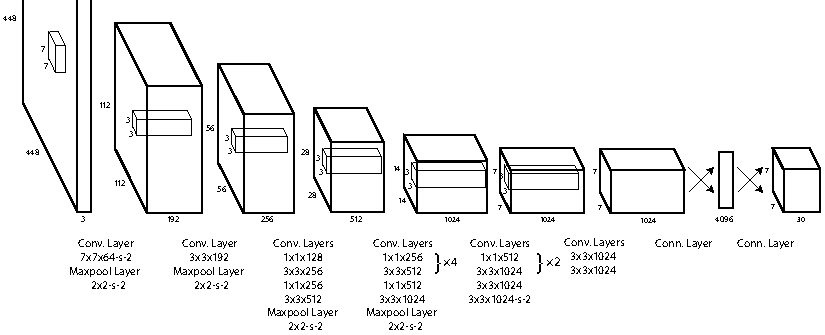
\includegraphics[width=0.90\linewidth]{rys_ok/Yolov1Struct.pdf} 
%            \caption{Struktura sieci Yolo \cite{yolov1}}
%\end{figure} 


\subsection{Yolo v2}
Detektor obiektów YOLO v2 wykorzystuje jednoetapową sieć detekcji obiektów. YOLO v2 jest szybszy niż dwuetapowe detektory obiektów z głębokim uczeniem, takie jak regiony z sieciami neuronowymi splotowymi (Faster R-CNN). Model YOLO v2 uruchamia sieć neuronową głębokiego uczenia (CNN) na obrazie wejściowym w celu wygenerowania predykcji sieciowych. Detektor obiektów dekoduje predykcje i generuje pola ograniczające. \cite{yolov2Matlab}

Architektura Darknet-19. Aby przyspieszyć i zwiększyć wydajność modelu, YOLOv2 wprowadził nową architekturę o nazwie „Darknet 19”. Nazwa tej architektury pochodzi od 19 warstw splotowych. Dla porównania, oryginalny YOLOv1 miał 8,5 miliarda parametrów, podczas gdy Darknet 19 zredukował je do 5,5 miliarda. Darknet 19 jest nie tylko wydajny, ale i wydajny. Jeśli chodzi o klasyfikację obrazów, konkuruje z wiodącymi modelami, takimi jak VGG czy ResNet, zachowując jednocześnie wysoką prędkość 200 klatek na sekundę (FPS). Oryginalny YOLOv1 był już znany ze swojej szybkości i dokładności, a Darknet 19 bazuje na tym dziedzictwie. Modyfikacje wprowadzone w Darknecie 19 w zakresie wykrywania obiektów obejmują usunięcie ostatnich w pełni połączonych warstw i ostatecznej warstwy klasyfikacji. W ich miejsce dodano trzy warstwy splotowe, a następnie warstwę „przelotową”, o której mówiliśmy wcześniej. Ta warstwa przelotowa łączy mapy cech w określony sposób, tworząc ostateczną mapę cech o wymiarach 13x13x125, która służy do wykrywania obiektów \cite{yolov2medium}.

%\begin{figure}[ht]
%    	\centering 
%            \includegraphics[width=0.60\linewidth]{rys_ok/yolo2_sctuct1.jpg} 
%            \caption{Realizacja sieci Yolo2 struktura Darknet-19 \cite{yolov2medium}}
%\end{figure} 

%\begin{figure}[ht]
%    	\centering 
%            \includegraphics[width=0.95\linewidth]{rys_ok/Yolo2_struct2.jpg} 
%            \caption{Realizacja sieci Yolo2 struktura Darknet-19 \cite{yolov2medium}}
%\end{figure} 



\subsection{Yolo v3}
Detektor obiektów YOLO v3 to wieloskalowa sieć detekcji obiektów, która wykorzystuje sieć ekstrakcji cech i wiele głowic detekcyjnych do tworzenia prognoz w wielu skalach. Model detekcji obiektów YOLO v3 uruchamia na obrazie wejściowym splotową sieć neuronową (CNN) z głębokim uczeniem, aby generować prognozy sieciowe z wielu map cech. Detektor obiektów gromadzi i dekoduje prognozy, aby generować pola ograniczające. YOLO v3 do prognozowanie obiektów na obrazie w używa pól zakotwiczenia, przewiduje te trzy atrybuty dla każdego pola zakotwiczenia.
przecięcie przez sumę (IoU), przesunięcia pól zakotwiczenia i prawdopodobieństwo klasy - etykietę klasy przypisaną do każdego pola zakotwiczenia.  \cite{yolov3Matlab}

\begin{figure}[ht]
    	\centering 
            \includegraphics[width=0.8\linewidth]{rys_ok/yolo3_struct.jpg} 
            \caption{YOLO-V3 budowa \cite{yolov3Matlab}}
\end{figure} 

\begin{figure}[ht]
    	\centering 
            \includegraphics[width=0.8\linewidth]{rys_ok/yolo3arch.jpg} 
            \caption{YOLO-V3 struktura źródło: Uri Almog \cite{yolov3Uri}}
\end{figure} 


\subsection{Yolo v4}
Sieć detekcji obiektów YOLO v4 to jednoetapowa sieć detekcji obiektów, składająca się z trzech części: szkieletu (backbone), szyi (neck) i podstawy (head). Szkielet może być wstępnie wytrenowaną splotową siecią neuronową, taką jak VGG16 lub CSPDarkNet53, trenowaną na zbiorach danych COCO lub ImageNet. Szkielet sieci YOLO v4 pełni funkcję sieci ekstrakcji cech, która oblicza mapy cech z obrazów wejściowych.
Szyja (neck) łączy szkielet z podstawą. Składa się ona z modułu puli piramid przestrzennych (SPP) i sieci agregacji ścieżek (PAN). Szyja (neck) łączy mapy cech z różnych warstw sieci szkieletowej i przesyła je jako dane wejściowe do podstawy (head).
Podstawa (head) przetwarza zagregowane cechy i przewiduje pola ograniczające, wyniki obiektowości i wyniki klasyfikacji. Sieć YOLO v4 wykorzystuje jednoetapowe detektory obiektów, takie jak YOLO v3, jako głowice detekcyjne.
Moduł SPP w szyjce łączy dane wyjściowe funkcji max-pooling mapy cech o niskiej rozdzielczości w celu ekstrakcji najbardziej reprezentatywnych cech. Moduł SPP wykorzystuje jądra o rozmiarach 1x1, 5x5, 9x9 i 13x13 do operacji max-pooling. Wartość kroku jest ustawiona na 1. Łączenie map cech zwiększa pole odbioru cech szkieletu i zwiększa dokładność sieci w wykrywaniu małych obiektów. Połączone mapy cech z modułu SPP są łączone z mapami cech o wysokiej rozdzielczości za pomocą modułu PAN. Moduł PAN wykorzystuje operacje upsamplingu i downsamplingu do wyznaczania ścieżek od dołu do góry i od góry do dołu, łącząc cechy niskiego i wysokiego poziomu.
Moduł PAN generuje zestaw zagregowanych map cech do wykorzystania w predykcjach. Sieć YOLO v4 ma trzy głowice detekcyjne. Każda głowica detekcyjna to sieć YOLO v3, która oblicza ostateczne predykcje. Sieć YOLO v4 generuje mapy cech o rozmiarach 19x19, 38x38 i 76x76, aby przewidywać pola ograniczające, wyniki klasyfikacji i wyniki obiektowości.
Tiny YOLO v4 to lekka wersja sieci YOLO v4 z mniejszą liczbą warstw sieciowych. Tiny YOLO v4 wykorzystuje sieć piramidy cech jako szyję i ma dwie głowice detekcyjne YOLO v3. Wyjścia sieciowe zawierają mapy o rozmiarach 13x13 i 26x26, służące do obliczania prognoz.
\cite{yolov4Matlab}
\begin{figure}[ht]
    	\centering 
            \includegraphics[width=0.8\linewidth]{rys_ok/yolov4architecture.jpg} 
            \caption{YOLO-V4\cite{yolov4Matlab}}
\end{figure} 



\subsection{Yolo v5}
Ultralytics YOLOv5 to najnowocześniejszy, najnowocześniejszy (SOTA) model widzenia komputerowego opracowany przez Ultralytics . Oparty na frameworku PyTorch , YOLOv5 słynie z łatwości obsługi, szybkości i dokładności. Wykorzystuje on wnioski i najlepsze praktyki z szeroko zakrojonych badań i rozwoju, co czyni go popularnym wyborem do szerokiego zakresu zadań sztucznej inteligencji w zakresie widzenia, w tym wykrywania obiektów , segmentacji i klasyfikacji obrazów (https://docs.ultralytics.com/yolov5/)\cite{ultralytics_doc}.
Yolo w wersji 5 nie występuje natywnie dla Matlab.

\subsection{Meituan Yolo v6}
Meituan YOLOv6 to najnowocześniejszy detektor obiektów, który oferuje niezwykłą równowagę między szybkością a dokładnością, co czyni go popularnym wyborem w aplikacjach czasu rzeczywistego. Model ten wprowadza kilka istotnych ulepszeń w architekturze i schemacie treningowym, w tym implementację modułu konkatenacji dwukierunkowej (BiC), strategię treningu wspomaganego kotwicą (AAT) oraz ulepszoną konstrukcję szkieletu i szyi, zapewniającą najwyższą dokładność w zbiorze danych COCO. Diagram architektury modelu przedstawiający przeprojektowane komponenty sieciowe i strategie treningowe, które doprowadziły do znacznej poprawy wydajności. (a) Szyja YOLOv6 (pokazano N i S). Uwaga: w przypadku M/L, RepBlocks jest zastępowany przez CSPStackRep. (b) Struktura modułu BiC. (c) Blok SimCSPSPPF. Moduł konkatenacji dwukierunkowej (BiC): YOLOv6 wprowadza moduł BiC w szyjce detektora, wzmacniając sygnały lokalizacji i zapewniając wzrost wydajności przy pomijalnym spadku prędkości. Strategia treningu wspomaganego kotwicą (AAT): Ten model proponuje AAT korzystanie z zalet zarówno paradygmatów opartych na kotwicy, jak i bez kotwicy, bez obniżania wydajności wnioskowania. Ulepszona konstrukcja szkieletu i szyjki: Dzięki pogłębieniu YOLOv6 o kolejny etap w szkielecie i szyjce, model ten osiąga najnowocześniejszą wydajność w zbiorze danych COCO przy wejściu o wysokiej rozdzielczości.\cite{ultralytics_doc}.
\begin{figure}[ht]
    	\centering 
            \includegraphics[width=0.95\linewidth]{rys_ok/yolo6struct.jpg} 
            \caption{YOLO-V6\cite{ultralytics_doc}}
\end{figure} 
Yolo w wersji 6 nie występuje natywnie dla Matlab.


\subsection{Yolo v7}
YOLOv7 to najnowocześniejszy detektor obiektów w czasie rzeczywistym, który przewyższa wszystkie znane detektory obiektów zarówno szybkością, jak i dokładnością w zakresie od 5 do 160 klatek na sekundę. Ma najwyższą dokładność (56,8\% AP) spośród wszystkich znanych detektorów obiektów w czasie rzeczywistym z 30 klatkami na sekundę lub więcej na GPU V100. Co więcej, YOLOv7 przewyższa inne detektory obiektów, takie jak YOLOR, YOLOX, Scaled-YOLOv4, YOLOv5 i wiele innych pod względem szybkości i dokładności. Model jest trenowany od podstaw na zbiorze danych MS COCO, bez użycia innych zbiorów danych ani wstępnie wytrenowanych wag.  

Wykrywanie obiektów w czasie rzeczywistym jest ważnym elementem wielu systemów widzenia komputerowego, w tym śledzenia wielu obiektów, autonomicznej jazdy, robotyki i analizy obrazów medycznych. W ostatnich latach rozwój detekcji obiektów w czasie rzeczywistym koncentrował się na projektowaniu wydajnych architektur i zwiększaniu szybkości wnioskowania różnych procesorów (CPU), procesorów graficznych (GPU) i neuronowych jednostek przetwarzania (NPU). YOLOv7 obsługuje zarówno mobilne procesory graficzne (GPU), jak i urządzenia GPU, od krawędzi sieci po chmurę.
W przeciwieństwie do tradycyjnych detektorów obiektów w czasie rzeczywistym, które koncentrują się na optymalizacji architektury, YOLOv7 koncentruje się na optymalizacji procesu uczenia. Obejmuje to moduły i metody optymalizacji zaprojektowane w celu zwiększenia dokładności wykrywania obiektów bez zwiększania kosztów wnioskowania, co jest koncepcją znaną jako treningowy „worek-rzeczy”.

\subsection{Yolo v8}
YOLOv8 został wydany przez Ultralytics 10 stycznia 2023 roku, oferując najnowocześniejszą wydajność pod względem dokładności i szybkości. Opierając się na udoskonaleniach poprzednich wersji YOLO, YOLOv8 wprowadził nowe funkcje i optymalizacje, które czynią go idealnym wyborem do różnych zadań wykrywania obiektów w szerokim zakresie zastosowań\cite{ultralytics_doc}.
\begin{figure}[ht]
    	\centering 
            \includegraphics[width=0.5\linewidth]{rys_ok/yolo8.jpg} 
            \caption{YOLO V8\cite{yolov8ar}}
\end{figure} 

Implementacja Yolo8 dla Matlab
To repozytorium oferuje różnorodne, wstępnie wytrenowane sieci YOLO v8 do wykrywania obiektów i segmentacji instancji w MATLAB®. Sieci te są trenowane na zbiorze danych COCO 2017[2] i umożliwiają wykrywanie 80 różnych kategorii obiektów, w tym osób, samochodów, sygnalizacji świetlnej itp. Ponadto repozytorium obsługuje trenowanie niestandardowych detektorów obiektów w celu precyzyjnego dostrojenia modeli do konkretnych zastosowań.
Oprogramowanie i wagi modeli są udostępniane na licencji GNU Affero General Public License v3.0.\cite{yolov8Matlab} 

\subsection{Yolo v9}
YOLOv9 to znaczący postęp w dziedzinie wykrywania obiektów w czasie rzeczywistym, wprowadzając przełomowe techniki, takie jak programowalna informacja gradientowa (PGI) i uogólniona efektywna sieć agregacji warstw (GELAN). Model ten charakteryzuje się znaczną poprawą wydajności, dokładności i adaptacyjności, wyznaczając nowe standardy w zbiorze danych MS COCO. Projekt YOLOv9, choć rozwijany przez odrębny zespół open source, opiera się na solidnej bazie kodu dostarczonej przez Ultralytics YOLOv5, co świadczy o duchu współpracy społeczności badawczej zajmującej się sztuczną inteligencją.

\begin{figure}[ht]
    	\centering 
            \includegraphics[width=0.8\linewidth]{rys_ok/yolo9.jpg} 
            \caption{YOLO V9\cite{yolov9}}
\end{figure} 

Informacje o implementacji modelu Yolo v9 dla Matlab\cite{yolov9matlab}




\subsection{Yolo v10}
Yolo v10 oparty na pakiecie Ultralytics Python, opracowany przez naukowców z Uniwersytetu Tsinghua, wprowadza nowe podejście do wykrywania obiektów w czasie rzeczywistym, rozwiązując zarówno problemy związane z postprocessingiem, jak i architekturą modelu, które wystąpiły we wcześniejszych wersjach YOLO. Dzięki wyeliminowaniu tłumienia niemaksymalnego (NMS) i optymalizacji różnych komponentów modelu, YOLOv10 osiąga najwyższą wydajność przy znacznie zmniejszonym narzucie obliczeniowym. Obszerne eksperymenty wykazują korzystny kompromis między dokładnością a opóźnieniem w wielu skalach modelu. \cite{ultralytics_doc}

\begin{figure}[ht]
    	\centering 
            \includegraphics[width=0.8\linewidth]{rys_ok/yolo10.jpg} 
            \caption{YOLO V10\cite{ultralytics_doc}}
\end{figure} 
Yolo w wersji 6 nie występuje natywnie dla Matlab.

\subsection{Yolo v11}
YOLO11 to najnowsza wersja detektorów obiektów w czasie rzeczywistym z serii Ultralytics YOLO, która na nowo definiuje możliwości dzięki najnowocześniejszej dokładności, szybkości i wydajności. Opierając się na imponujących postępach poprzednich wersji YOLO, YOLO11 wprowadza znaczące ulepszenia w architekturze i metodach uczenia, czyniąc go wszechstronnym wyborem do szerokiego zakresu zadań z zakresu wizji komputerowej.YOLO11 wykorzystuje ulepszoną architekturę szkieletową i szyjową, która rozszerza możliwości ekstrakcji cech, zapewniając precyzyjniejsze wykrywanie obiektów i wydajność złożonych zadań. YOLO11 wprowadza udoskonalone projekty architektoniczne i zoptymalizowane procesy szkoleniowe, zapewniając większą prędkość przetwarzania i zachowując optymalną równowagę między dokładnością a wydajnością.
Większa dokładność przy mniejszej liczbie parametrów: Dzięki ulepszeniom w projektowaniu modeli, YOLO11m osiąga wyższą średnią precyzję (mAP) w zbiorze danych COCO, wykorzystując o 22\% mniej parametrów niż YOLOv8m, co zapewnia wydajność obliczeniową bez utraty dokładności.YOLO11 można bezproblemowo wdrożyć w różnych środowiskach, w tym na urządzeniach brzegowych, platformach chmurowych i systemach obsługujących procesory graficzne NVIDIA, co zapewnia maksymalną elastyczność. Szeroki zakres obsługiwanych zadań: Niezależnie od tego, czy chodzi o wykrywanie obiektów, segmentację instancji, klasyfikację obrazów, estymację pozycji, czy zorientowane wykrywanie obiektów (OBB), YOLO11 został zaprojektowany z myślą o zróżnicowanym zestawie wyzwań związanych z przetwarzaniem obrazu.\cite{yolov11}

\begin{figure}[ht]
    	\centering 
            \includegraphics[width=0.4\linewidth]{rys_ok/yolo11.jpg} 
            \caption{YOLO V10\cite{yolov11medium}}
\end{figure} 
Yolo w wersji 11 nie występuje natywnie dla Matlab.


\subsection{Yolo 12}
Architekturę skoncentrowaną na uwadze, która odchodzi od tradycyjnych podejść opartych na sieciach neuronowych (CNN) stosowanych w poprzednich modelach YOLO, zachowując jednocześnie szybkość wnioskowania w czasie rzeczywistym, niezbędną w wielu zastosowaniach. Model ten osiąga najnowocześniejszą dokładność wykrywania obiektów dzięki nowatorskim innowacjom metodologicznym w mechanizmach uwagi i ogólnej architekturze sieci, zachowując jednocześnie wydajność w czasie rzeczywistym.
Mechanizm uwagi obszarowej: Nowe podejście do samouważności, które efektywnie przetwarza duże pola recepcyjne. Dzieli mapy obiektów na l obszarów o równej wielkości (domyślnie 4), poziomo lub pionowo, unikając skomplikowanych operacji i utrzymując duże efektywne pole recepcyjne. To znacznie zmniejsza koszty obliczeniowe w porównaniu ze standardową samouważnością.[...]
Implementacja Ultralytics YOLO12 domyślnie nie wymaga FlashAttention. FlashAttention można jednak opcjonalnie skompilować i używać z YOLO12. Do kompilacji FlashAttention potrzebny jest jeden z następujących procesorów graficznych NVIDIA:
\begin{itemize}
    \item GPU Turing (np. seria T4, Quadro RTX)
    \item GPU Ampere (np. seria RTX30, A30/40/100)
    \item GPU Ada Lovelace (np. seria RTX40)
    \item GPU Hopper (np. H100/H200) \cite{ultralytics_doc}.
\end{itemize}

\begin{figure}[ht]
    	\centering 
            \includegraphics[width=0.9\linewidth]{rys_ok/yolov12_vs_prev.png} 
            \caption{YOLO wersje wcześniejsza a wersja 12\cite{yolov12}}
\end{figure} 


\section{Wdrożenie Yolo w Matlab}

Uruchomienie modeli Yolo w wersjach oraz 2, 3, 4 oraz 8 dostępne jest poprzez instalację odpowiednich rozszerzeń. \cite{yolov2Matlab} \cite{yolov3Matlab} \cite{yolov4Matlab} \cite{yolov8Matlab}.

Zdjęcia użyte w kodzie pochodzą z 
\cite{imagedog},
\cite{imagedog2}



%https://www.mathworks.com/matlabcentral/fileexchange/179569-object-detection-and-instance-segmentation-using-yolo-v8?s_tid=srchtitle_support_results_1_yolo+v8
%v8:
% Load YOLO v8 model
%det = yolov8ObjectDetector('yolov8s');

% Analyze loaded model
%analyzeNetwork(det.Network);

    %\chapter{Środowiska}
    %% W drugiej części opisano i porównano warunki budowania środowisk.

    %\chapter{Model perceprtonu wielowarstwowego MLP}
    %\begin{figure}[ht]
	\centering 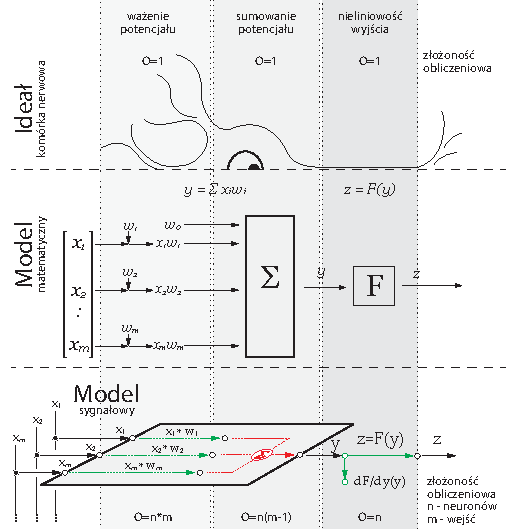
\includegraphics[width=0.9\linewidth]{rysunki/stan_wiedzy_1.jpg} 
	\caption{ Neuron, model matematyczny i sygnałowy  }
	\label{rys:neuronmodel1}
\end{figure}
%ideał - równoległego przetwarzania
%dwukrotne zwiększenie liczby wejść nie powoduje zwiększenia czasu przetwarzania. 
%krok pierwszy: realizacja niezależnego równoległego "ważenia" x1w = x1*w1, x2w = x2*w2, x3w=w3*w3 ... mnożenie o złożoności obliczeniowej: O=1;
%krok drugi: realizacja równoległego wielokanałowego dodawania. sum = x1w + x2w + x3w ..; dodawanie o złożoności obliczeniowej O=1;
%krok trzeci: aktywacja nieliniowa aktywacja F;
Neuron biologiczny przetwarza impulsy wejściowe w trzech krokach:
\begin{itemize}
    \item 
    ważenie wejściowych sygnałów - jest to skomplikowany proces, zmienny w czasie i zależny od historii wcześniejszych impulsów; w modelu matematycznym odpowiada mu mnożenie sygnału wejściowego \(x_i\) przez wielkość wagi \(w_i\) przypisanej do tego sygnału. \( x_iw = x_i * w_i  \)
    
    \item 
    jednoczesne sumowanie potencjałów sygnałów wejściowych - w modelu matematycznym odpowiada mu algebraiczna suma ważonych sygnałów: \( y = \sum x_iw \)

    \item 
    nieliniowa aktywacja - w modelu matematycznym obliczenie wartości funkcji aktywacji \( z = F(y) \)

    \item w modelu sygnałowym dla zwiększenia wydajności zapamiętano wartość pochodnej \(  \frac{\partial F}{\partial y}(z) \) -~zostanie ona wykorzystana w późniejszych obliczeniach w procesie uczenia.
    
\end{itemize} 
 
%W tym rozdziale autor opisze stan wiedzy - matematyczny i sygnałowy model warstwy splotowej CNN oraz warstwy MLP głównych elementów składowych sieci głębokich. A także działanie warstw pomocniczych - łączących, i redukujących. 
%Opisany będzie sposób obliczania odpowiedzi sieci na zaprezentowany wzór - tj. przepływ sygnału wprost. 
%Ponadto opisany zostanie algorytm uczenia "wsteczna propagacją błędu" jako operacja matematyczna i proces przesyłania sygnału wstecz przez sieć.

%*******************
 




\begin{center}
\begin{tabular}{|c|c|c|} 
 \hline
 rodzaj warstwy & funkcja aktywacji  \(  z = F(y) \)  & wartość pochodnej \(  \frac{\partial F}{\partial y} \) \\ 
 logistyczna (sigmoid) &  \( \frac{1}{1+e^-y} \) & \( (z)(1-z) \) \\ 
 ReLU & jeśli y<0 to z=y, jeśli y>=0 to z=0  & jeśli y<0 to 1, jeśli y>=0 to 0 \\ 
  softmax &   \(z_i = \frac{e^{x_i}}{\sum{e^{x_i}}}   \) & dla prawidłowej klasy k:  \(y_k(1-y_k)\),     \\
 softmax &  &  dla pozostałych klas:  \(  -y_i*y_k  \) \\

 \hline 
\end{tabular}
\end{center}


\section{Perceptron warstwowy}
Wejście neuronu przyjmuje wartości  \([ x_1, x_2,  ... , x_m ]\) (wektor), natomiast na wyjściu jednego neuronu pojawia się tylko jeden sygnał wyjściowy \(z\). 
\begin{figure}[ht]
	\centering 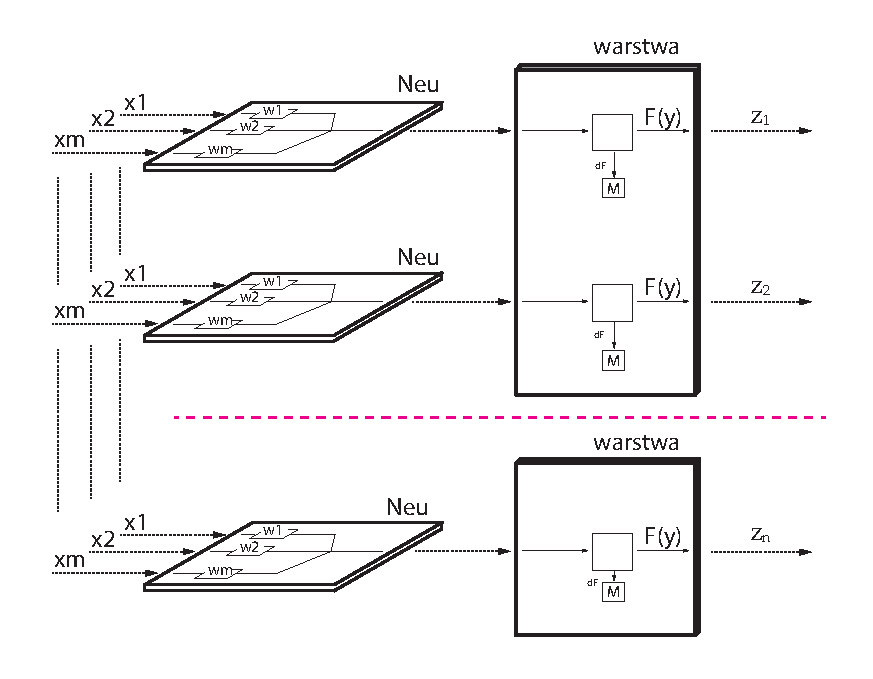
\includegraphics[width=0.75\textwidth]{rysunki/3d.jpg} 
\caption{Przepływ sygnałów przez warstwę w czasie propagacji sygnału "w przód" }
	\label{rys:modelobiektowegoneuronuszkic3}
\end{figure}
 

\begin{figure}[ht]
	\centering \includegraphics[width=0.60\textwidth]{rysunki/forward_layers.jpg} 
	\caption{Propagacja sygnału przez zespół warstw w przód i wstecz}
	\label{rys:operacjesynch2a}
\end{figure}

\section{Proces uczenia MLP}
\begin{figure}[ht]
	\centering 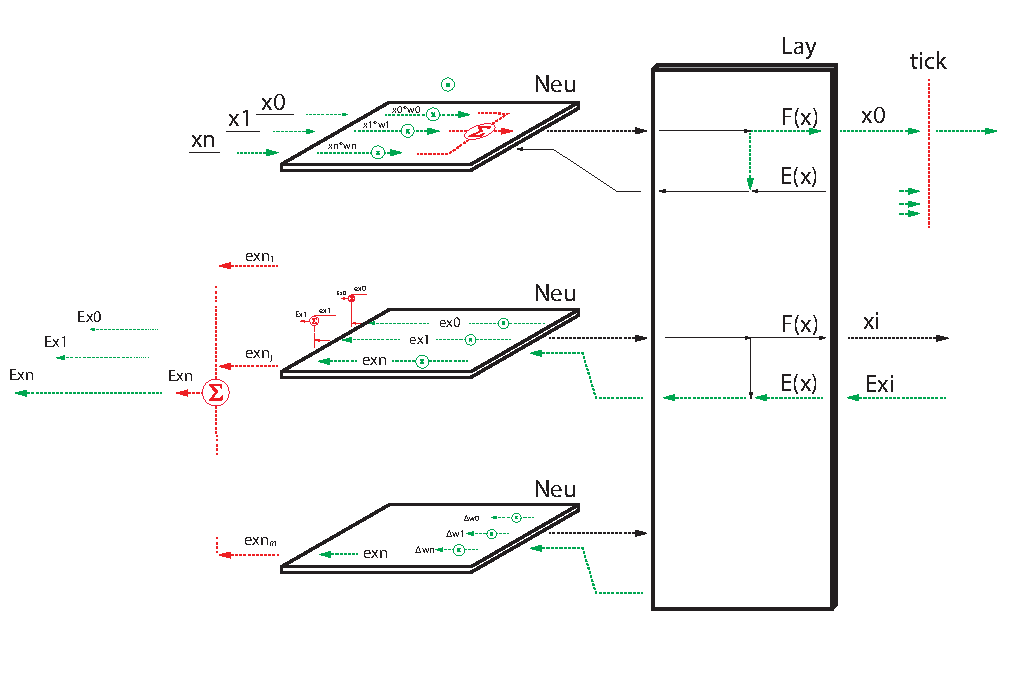
\includegraphics[width=0.93\textwidth]{rysunki/3drev.jpg} 
	\caption{Propagacja wstecz - uczenie sieci. (Operacje niezależne (mnożenie) oznaczone kolorem zielonym i operacje wymagające synchronizacji (dodawanie) oznaczone kolorem czerwonym)}
	\label{rys:operacjesynch2}
\end{figure}
Odpowiedzią sieci jest sygnał wyjściowy ostatniej warstwy. W procesie uczenia z nauczycielem podlega on ocenie, a wielkość błędu sieci jest przekazywana do warstwy wyjściowej. Stosowane są różne strategie wyznaczania wielkości tego wektora. \\
Dla warstwy wyjściowej logistycznej może to być różnica między oczekiwaną odpowiedzią, a odpowiedzią uzyskaną:
\( \left[
                        \begin{matrix}
                             e_{1}\\
                             e_{2}\\
                             e_{m}\\
                        \end{matrix}
                    \right]
                    = 
                     \left[
                        \begin{matrix}
                             s_{1}\\
                             s_{2}\\
                             s_{m}\\
                        \end{matrix}
                    \right]
                    -
                    \left[
                        \begin{matrix}
                             z_{1}\\
                             z_{2}\\
                             z_{m}\\
                        \end{matrix}
                    \right]
\)  gdzie \(S\) jest wektorem oczekiwanym.  
Dla każdej wartości wyjściowej \(z_i\) zostaje zwrócona wielkość błędu \(e_i\), ponadto dla każdej wartości~\(z_i\) zostaje zapamiętana wartość pochodnej \(  \frac{\partial F}{\partial y} \). W procesie uczenia do każdego z neurosumatorów zostaje przekazana odpowiadająca mu wielkość błędu: \( dFe = e_i *  \frac{\partial F}{\partial y} \).  \\
\begin{figure}[ht]
	\centering 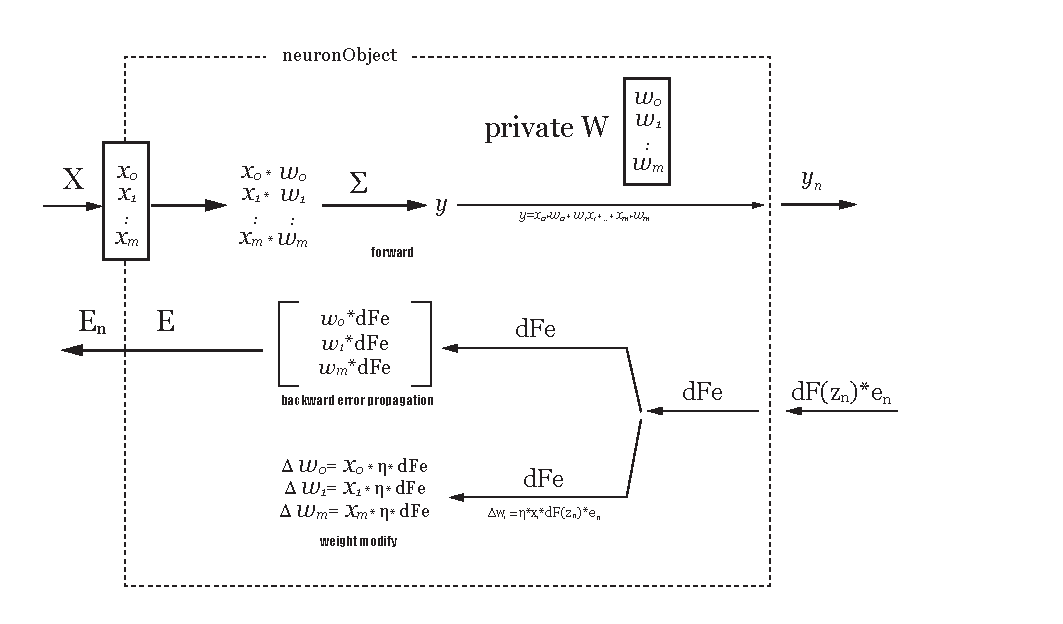
\includegraphics[width=\textwidth]{rysunki/rys1_5.jpg} 
	\caption{Przepływu sygnałów w obiekcie Neurosumator }
	\label{rys:modelobiektowegoneuronuszkic2}
\end{figure}


    %\chapter{Model sieci głębokiej CNN}
    %\section{Wstęp}
Za protoplastę tych (głębokich) sieci można uznać zdefiniowany na początku lat `90 wielowarstwowy neocognitron prof. Kunihiko Fukushimy. Prawdziwy rozwój tych sieci zawdzięczamy jednak profesorowi Yann A. LeCun, który zdefiniował podstawową strukturę i algorytm uczący specjalizowanej sieci konwolucyjnej CNN. Aktualnie sieci CNN stanowią podstawową strukturę stosowaną na szeroką skalę w przetwarzaniu sygnałów i obrazów. W międzyczasie powstało wiele odmian sieci będącej modyfikacją struktury podstawowej (R-CNN, AlexNET, GoogLeNet, ResNet, U-Net, YOLO)\cite{Osowski2023}.\\
Sieci CNN powstały jako narzędzie analizy i rozpoznawania obrazów wzorowanym na sposobie działania naszych zmysłów. Wyeliminowały kłopotliwy proces manualnego opisu cech charakterystycznych obrazów. W tym rozwiązaniu sieć sama odpowiada za generację cech charakterystycznych dla klas \cite{Osowski2023}. Przetwarzania obrazu przez zestaw filtrów i warstw generuje obrazy o coraz mniejszych  wymiarach, lecz o zwiększającej się liczebności kanałów reprezentujących cechy charakterystyczne dla przetwarzanego zbioru. Próbka danych w kolejnych etapach jest reprezentowana przez tensory (struktury trójwymiarowe, których szerokość i wysokość odpowiada wymiarom obrazu, a głębokość jest równa liczbie kanałów w obrazie). Wyjście z ostatniej warstwy sieci w procesie wypłaszczania jest przetwarzane na postać wektorową (jednowymiarowa tablica liczb), a następnie przekazywane na wejście układu klasyfikującego - sieci MLP z wyjściem Softmax \cite{YannCnn} \cite{Qi2016DerivationOB}.


%\href{2016.10 - Derivation of Backpropagation in Convolutional Neural Network (CNN).pdf}

%\href{https://zzutk.github.io/docs/reports/2016.10%20-%20Derivation%20of%20Backpropagation%20in%20Convolutional%20Neural%20Network%20(CNN).pdf}

%\href{https://www.bibsonomy.org/bibtex/28d520c74cb5aeee1bcae26642b7d973d/tobias.koopmann}



%Convolution !
%\href{https://arxiv.org/pdf/1603.07285}


%Back convolution
%\href{https://hal.science/hal-04409232/document}

~
\newline
\begin{figure}[ht]
    	\centering 
            \includegraphics[width=0.90\linewidth]{rysunki/Lecun98-7.jpg} 
            \caption{Architektura LaNet-5 \cite{YannCnn}}
\end{figure} 
\newpage 
\begin{figure}[ht]
    	\centering 
            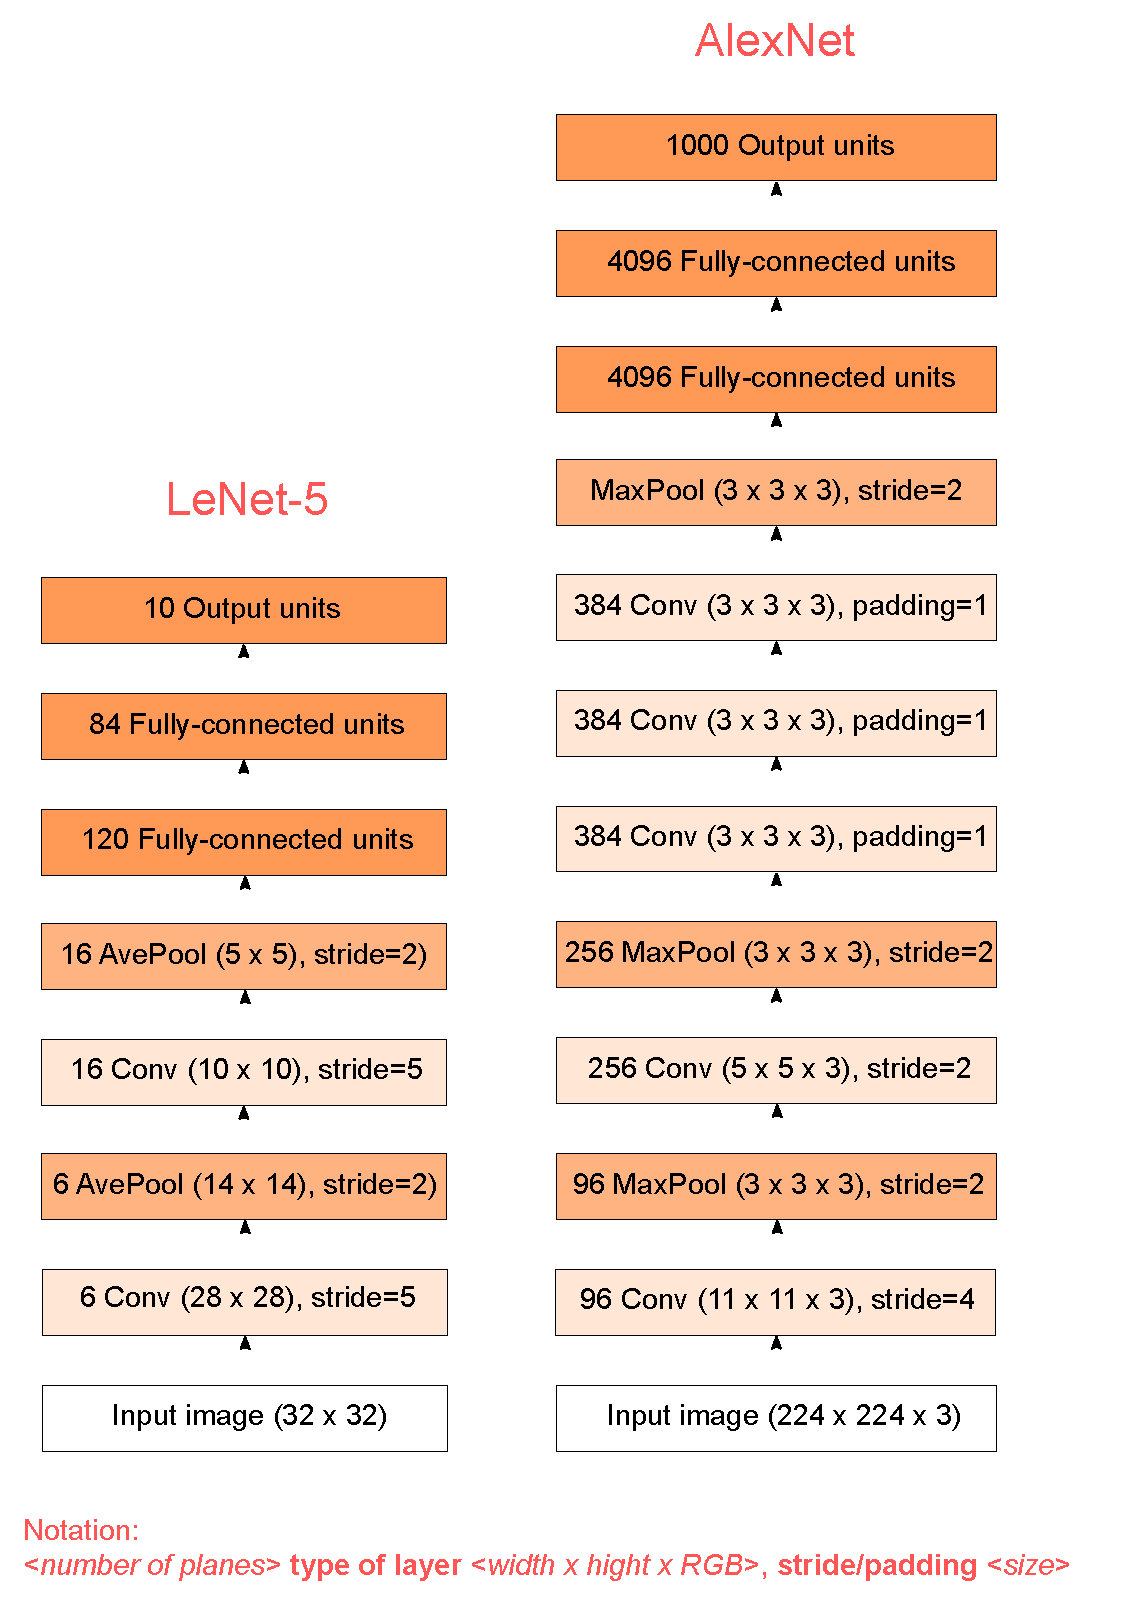
\includegraphics[width=0.70\linewidth]{rysunki/alexnet.jpg} 
            \label{fig:lanet}
            \caption{Porównanie struktury LaNet i AlexNet \cite{strAlexnet} }
\end{figure} 
\newpage 

 
\section{Operacja splotu }
Jeśli wartości pikseli obrazu wejściowego \(X\)
oznaczymy \(X_{(i,j)}\), a wartości filtra \(F\) oznaczymy jako \(F_{(m,n)}\) obraz wejściowy \(Y\), \(Y_{(o,p)}\), wówczas każdy piksel obrazu wyjściowego obliczymy:

\begin{equation}
      Y_{(O,P)} = \sum _{(n=1)} ^{(N)} 
                  \sum _{(m=1)} ^{(M)} 
                  F_{(m,n)}*X_{(m+O,n+P)}
\end{equation} 

\begin{figure}[ht]
    	\centering 
            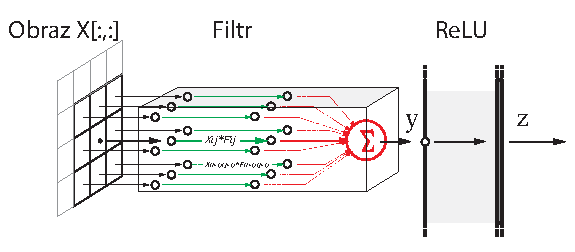
\includegraphics[width=0.70\linewidth]{rysunki/rys2_1.jpg} 
            \caption{Obliczanie wartości pojedynczego piksela w procesie splotu analogicznie jak w MLP, sprowadza się do obliczenia sumy ważonej piksela centralnego filtra z pikselem obrazu oraz najbliższych sąsiadów centralnego piksela - tych które znajdują się naprzeciw pikseli filtra. }
\end{figure} 
\subsection{Padding}

\begin{figure}[ht]
    	\centering 
            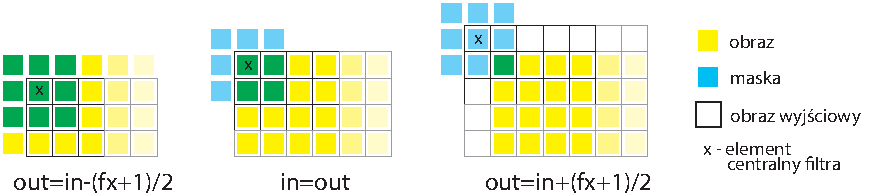
\includegraphics[width=0.99\linewidth]{rysunki/rys2_2.jpg} 
            \caption{Wpływ punktu startowego maski na wymiar obrazu wynikowego operacji splotu }
\end{figure} 
Padding oznacza wysunięcie maski poza obszar obrazu. \newline Jeśli w procesie konwolucji centralny piksel maski:
\begin{itemize}
    \item 
    znajduje się przed granicą obrazu, wówczas obraz wynikowy będzie mniejszy (p>0).
    
    \item 
    znajduje się nad pierwszym pikselem obrazu, wówczas wielkość obrazu wyjściowego jest taka jak obrazu wejściowego (p=0).

    \item 
    znajduje się poza pikselem obrazu, wówczas wielkość obrazu wyjściowego będzie większa (p<0).
    
\end{itemize}

W założeniu procesu uczenia, każdy przesyłany sygnał wejściowy i wyjściowy jest sprzężony z powrotnym sygnałem określającym wielkość błędu tego sygnału. Zatem jeśli w operacji splotu padding jest dodatni, wówczas przy obliczeniu błędu wyjściowego zastosowany będzie padding ujemny.


\subsection{Stride}
%Stride oznacza skok o ile pikseli przesuwa się maska w jednym kroku.
\begin{figure}[ht]
    	\centering 
            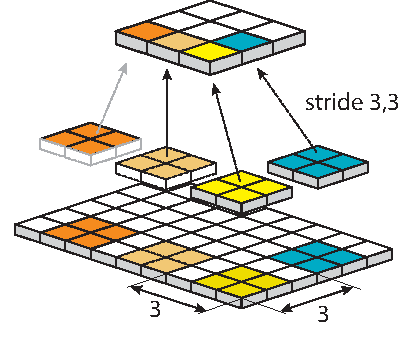
\includegraphics[width=0.4\linewidth]{rysunki/conv4a.jpg} 
            \caption{Stride, krok przesunięcia maski}
\end{figure} 

Wymiar wyjściowy obrazu  \(dimOut = ( dimIn + 1 - dimF + 2*padding ) / stride \) 
\begin{figure}[ht]
    	\centering 
            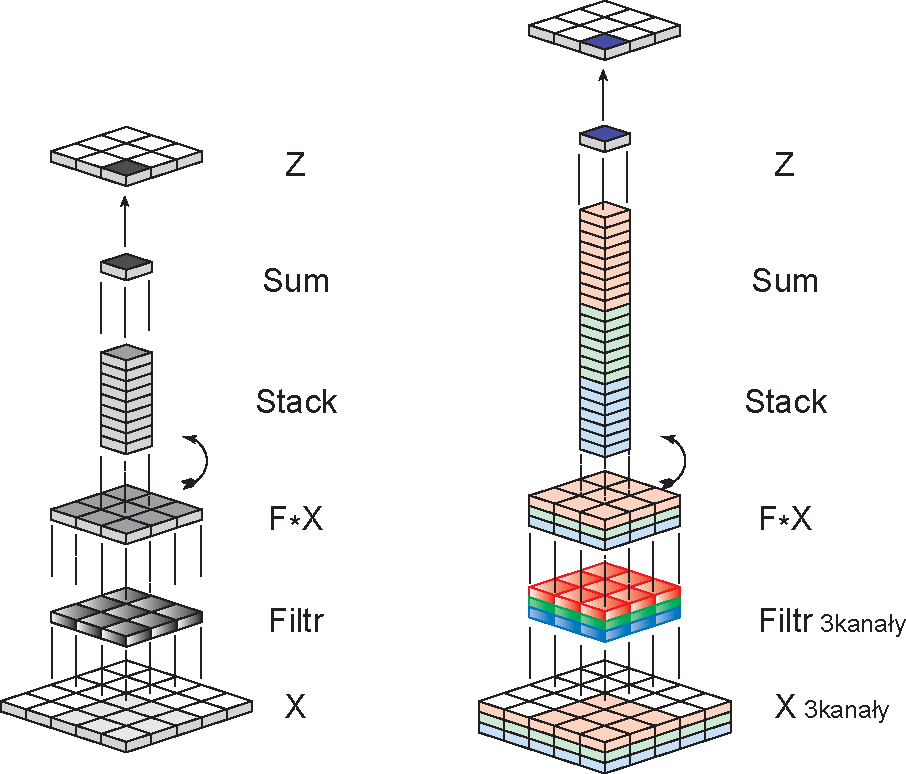
\includegraphics[width=0.76\linewidth]{rysunki/conv2b.jpg} 
            \caption{Konwolucja jedno i wielokanałowa}
\end{figure} 




\newpage
\section{ReLU i warstwy redukujące wymiar }

\begin{figure}[ht]
    	\centering 
            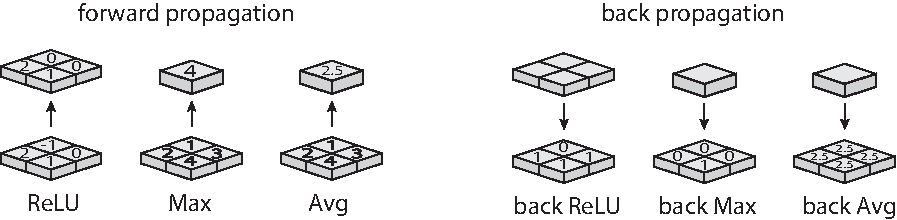
\includegraphics[width=0.95\linewidth]{rysunki/conv3.jpg} 
            \caption{Wynik działania warstw ReLU, Avg, Max przy przepływie wprost i wstecz.  }
\end{figure} 
Po operacji splotu można zastosować warstwę ReLU. Funkcja aktywacji ReLU = max\{x, 0\}. Zerowane są wartości ujemne, funkcja nie ma ciągłej pochodnej, przy obliczeniach przyjmowano że pochodna wynosi 1 gdy wartość wyjścia z była większa od 0, lub 0 jeśli wartość z była mniejsza od zera.\newline
Można także zastosować warstwy redukującą rozmiar. Warstwa AVG - na wyjściu zwraca średnią wartości sąsiednich pól; pochodna przy przepływie wstecz dla każdego pola wynosi \(1/n^2\) gdzie n jest wielkością filtra. Warstwa MAX - na wyjściu zwraca wartość maksymalną z pól objętych zasięgiem filtra. Pochodna przy propagacji wstecz wynosi 1 dla wartości maksymalnej i 0 dla pozostałych.  

\section{Przetwarzanie w przód }
Obraz wejściowy w skali szarości, lub obraz kolorowy rozbity na 3 kanały RGB zostaje przetworzony w operacji splotu przez grupy warstw filtrów i warstwy redukujące. Warstwa konwolucyjna może zmniejszyć, a warstwa redukująca zawsze zmniejsza rozmiar obrazu, w efekcie otrzymujemy coraz mniejsze obrazy wyjściowe. \newline
Wyjściem każdego filtra jest jeden kanał obrazu. W miarę zmniejszania obrazów stosowana jest większa liczbę filtrów, co zwiększa liczbę kanałów. Przedostatnia warstwa spłaszcza wszystkie kanały obrazu do postaci pojedynczego jednowymiarowego wektora, warstwa ostatnia Full Connected z~wyjściem Softmax dokonuje klasyfikacji obrazu.
 

\section{Przetwarzanie wstecz - modyfikacja filtra w warstwie splotowej }
Wektor wielkości błędu zostaje przekazany z warstw MLP przez warstwy redukujące do warstw splotowych, w których następuje modyfikacja Filtra zgodnie z formułą.

\begin{equation}
    \frac{\partial L}{\partial F} = Conv( Input.X , Loss.Gradient \frac{\partial L}{\partial O} ) ; 
    F=F-\mu * \frac{\partial L}{\partial F}
\end{equation}
\begin{equation}
    \frac{\partial L}{\partial Bias} = Sum( Loss.Gradient \frac{\partial L}{\partial O} ) ; 
    Bias=Bias-\mu * \frac{\partial L}{\partial Bias}
\end{equation}

\section{Propagacja błędu przez warstwę splotową }
Do warstwy poprzedniej zostanie przekazany wektor błędu o wartości wyliczonej wg. wzoru:

\begin{equation}
    \frac{\partial L}{\partial X} = FullConv( 180Rotated.filter.F, Loss.Gradient \frac{\partial L}{\partial O } )  
\end{equation}

    %\chapter{Szacowane obciążenie}
    %\input{tekst/szacowane_obciazenie}

    %\chapter{Problemy i skuteczne sposoby ich rozwiązywania}
    %%W rozdziale "wydajność" Autor przedstawi stosowane rozwiązania zwiększające wydajność sprzętową systemu, takie jak zestaw rozkazów MMX, AVX oraz możliwości kart graficznych GPU. 
%%
%Ponadto opisana będzie konieczność realizacji kluczowych operacji takich jak: równoległe mnożenie oraz wieloskładnikowe dodawania niezbędne do efektywnego budowania sieci MLP oraz CNN. 
%%
% ********************
\section{ Maszyna Turinga }
Zasada działania maszyny Turinga sprowadza się do cyklicznego wykonywania sekwencji operacji: odczytu wartości z pamięci, wykonaniu działania, zapisaniu wyniku w pamięci. Modelowanie tworu przetwarzającego informacje całą objętością przy użyciu maszyny sekwencyjnej w miarę powiększania modelu spowoduje lawinowy wzrost czasu przetwarzania.
%%
\section{ Szybsze obliczenia grafiki 3D }
W zastosowaniach inżynierskich (oraz rozrywkowych) maszyn liczących bardzo szybko pojawiała się potrzeba realizacji szybkich obliczeń translacji punktów w przestrzeni 3D.
Operacje te sprowadzają się do mnożenia wektora współrzędnych znormalizowanych punktu przez macierz translacji:
\begin{equation*} P =  \begin{bmatrix}
 x\\
 y\\
 z\\
 1
        \end{bmatrix} ,
  T =  \begin{bmatrix}
 1 & 0 & 0 & x\\
 0 & 1 & 0 & y\\
 0 & 0 & 1 & z\\
 0 & 0 & 0 & 1
        \end{bmatrix} ,
  O_x =  \begin{bmatrix}
 1 & 0 & 0 & 0\\
 0 & c & -s & 0\\
 0 & s & c & 0\\
 0 & 0 & 0 & 1
        \end{bmatrix} ,
R =  \begin{bmatrix}
 1 & 0 & 0 & 0\\
 0 & 1 & 0 & 0\\
 0 & 0 & 1 & 0\\
 0 & 0 & 1/d & 0
        \end{bmatrix} 
\end{equation*}

a po rozpisaniu mamy:
\begin{equation*}
\begin{matrix}
  X = x*m[0][0] + y*m[1][0]+z*m[2][0] + w*m[3][0] \\

  Y = x*m[0][1] + y*m[1][1]+z*m[2][1] + w*m[3][1] \\

  Z = x*m[0][2] + y*m[1][2]+z*m[2][2] + w*m[3][2] \\

  W = x*m[0][3] + y*m[1][3]+z*m[2][3] + w*m[3][3]  \\
  \end{matrix}
\end{equation*}
Pierwszą odpowiedzią na to zapotrzebowanie był wprowadzony na rynek w 1980 roku koprocesor arytmetyczny Intel 8087, jego zadaniem było przyspieszenie operacji arytmetycznych zwłaszcza na liczbach zmiennoprzecinkowych w systemach opartych o procesor Intel 8088 i Intel 8086.\newpage
\subsection{ Funkcje procesora MMX, SIMD, SSE, AVX }
SIMD (Single Instruction, Multiple Data) to funkcja procesora, która pozwala wykonywać jedną instrukcję na wielu 'strumieniach'  danych. Może ona ewentualnie zwiększyć wydajność Twoich programów. SIMD to postać przetwarzania równoległego; jednak w niektórych przypadkach przetwarzanie różnych strumieni może odbywać się sekwencyjnie. Pierwszą implementacją był zbiór instrukcji MMX, zastąpiony przez strumieniowe rozszerzenia SIMD (ang. Streaming SIMD Extension, SSE). Później do SSE dodano zaawansowane rozszerzenia wektorowe (ang. Advanced Vector Extension, AVX).\cite{asmx64} 
Procesor obsługujący SSE ma 16 dodatkowych rejestrów 128-bitowych (xmm0-xmm15). Procesor obsługujący AVX2 ma 256-bitowe rejestry ymm, AVX-256 i AVX-10 512-bitowe rejestry zmm.\cite{asmx64} 
\begin{figure}[ht]
	\centering 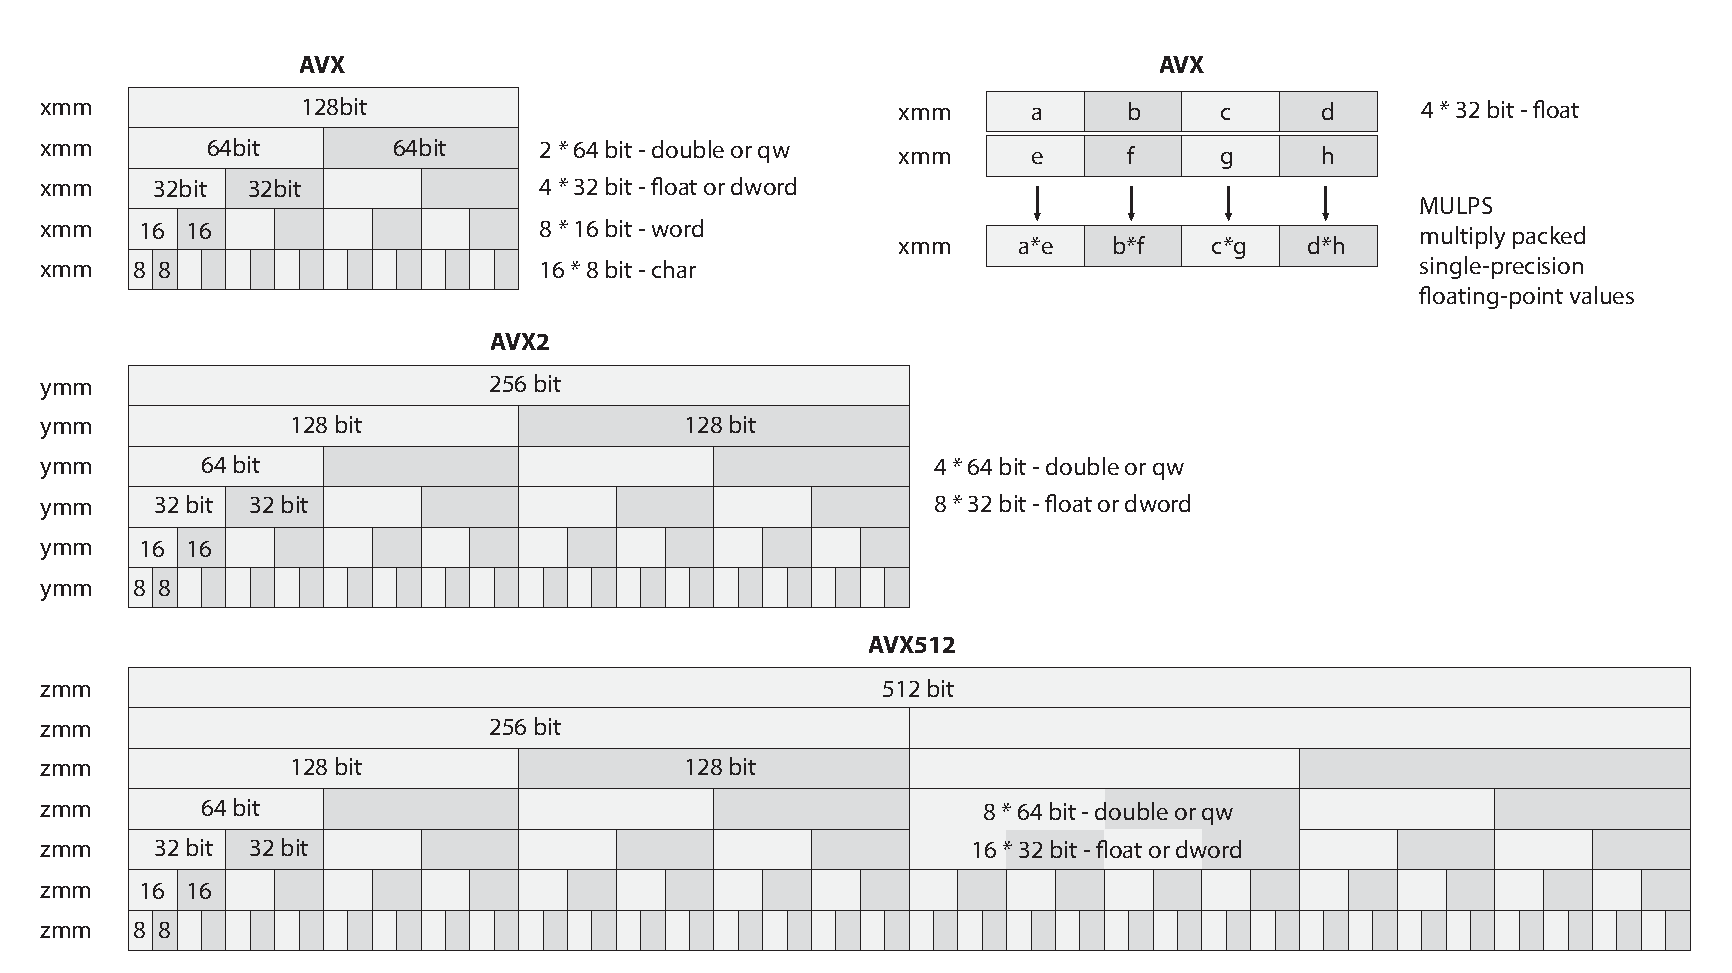
\includegraphics[width=0.99\textwidth]{rysunki/avx.jpg} 
	\caption{ Rejestry AVX, AVX2 i AVX512,operacja równoległego mnożenia AVX}
	\label{rys:modelsztucznegoneuronu}
\end{figure}
Rozkaz MULPS wykonuje jednocześnie jednocześnie 4 mnożenia zestawu 8 liczb 32 bitowych.\newline
Instrukcje w AVX512 VMPADDWD, VMPADDUBSW - wykonują mnożenie wektorowe, następnie dodawanie sąsiednich elementów. \((a_{i}\cdot b_{i}+a_{i+1}\cdot b_{i+1})\)

Funkcje te przyspieszają operacje iloczynu Hadamarda (.*)\cite{WKasprzak} czyli wielokanałowego mnożenia. W zależności od wersji dla zmiennych typu float uzyskano od 4 do 16 kanałów, czyli 16 operacji mnożenia w czasie jednego rozkazu.
\cite{yt_MMX}
\newpage
\section{ Obliczenia na GPU }
\subsection{Równoległe mnożenie}
Wydajne obliczanie iloczynu Hadamarda (.*) wektorów o dużych rozmiarach mogą zapewnić procesory graficzne, w których znajdują się tysiące jednostek obliczeniowych. Czas wykonania kilku tysięcy mnożeń zajmuje tyle samo czasu co wykonanie jednego mnożenia. Użycie kart graficznych przy modelowaniu głębokich sieci jest koniecznością, ponieważ skraca czas trenowania sieci o rzędy wielkości w stosunku do obliczeń na CPU. W niniejszej pracy wykorzystano kartę NVIDIA GeForce RTX 4070 wyposażonej w 5888 rdzeni CUDA oraz 12282 MB pamięci na karcie graficznej. \cite{cuda_} \cite{wroc}\newline
\begin{figure}[ht]
	\centering 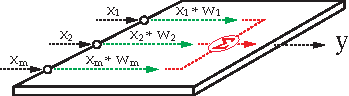
\includegraphics{rysunki/sum_2.jpg} 
	\caption{ Mnożenie równoległe i wielokanałowe dodawanie }
	\label{rys:operacje niezalezne i zalezne}
\end{figure}
\subsection{Wielokanałowe dodawanie}
Sumowanie a+b+c+d realizowane jest analogiczne do zdegenerowanego drzewa binarnego czyli 
(((a+b)+c)+d). Przy dużej ilości składników możemy spróbować zastosować zwykłe drzewo binarne niezdegenerowane, a operacja dodawania może stanie się częściowo równoległa ((a+b) + (c+d).
Maszyny cyfrowe obecnie nie są wyposażone w sumatory wielokanałowe pozwalające dodawać więcej niż 2 liczby jednocześnie. Można zasymulować quasi-równoległe dodawanie stosując nawiasy.
\begin{figure}[h]
	\centering 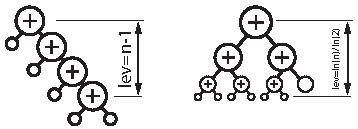
\includegraphics[width=0.6\textwidth]{rysunki/sum.jpg} 
	\caption{ drzewo zdegenerowane i niezdegenerowane}
	\label{rys:operacjesynch}
\end{figure}

\begin{itemize}
    \item \(b=((..((a1+a2)+(a3+a4))+((a5+a6) ...\) 
          czas wykonania: \textbf{0.09568 [sek.]}
    \item \( b=a1+a2+a3+a4+...+a1024\) 
          czas wykonania: \textbf{0.247875 [sek.]}    
\end{itemize}
~\newline
Uzyskamy dwukrotne zwiększenie szybkości przez dodanie nawiasów. Przy 32 składnikach mamy 16 + 8 + 4 + 2 + 1 dodawań, jednak pierwsze 16 może być wykonane równolegle, kolejna 8 także jest od siebie niezależna, podobnie 4 i 2. Czyli dla 32 elementów  mamy 31 dodawań w 5 poziomach. Dla 1024 składników mamy 1023 dodawania, 512+256+128...+1 w 10 poziomach. \cite{cuda_}
\section{Matlab}
Dodatek Parallel computing w Matlab umożliwia wykonywanie obliczeń równolegle, w osobnych wątkach, procesach, a także z wykorzystaniem kart graficznych (obecnie tylko NVidia). Dodatki Optimalization Toolbox i Optimalization Computing Toolbox optymalizują tworzony kod, zwiększając jego wydajność. Dodatek Deep Learning Toolbox dostarcza gotowych metod do obliczeń sieci neuronowych.
\newline
w Matlab karty graficzne (NVidia) są widoczne nawet bez instalowania w systemie dedykowanych sterowników. Karty AMD nie są widoczne.
 

    %\chapter{Zadania}
    %
% W tym rozdziale Autor opisze skrótowo zadania które wykonywały badane modele sieci, oraz zaprezentuje wyniki badań - czyli czasy realizacji zadania przez zbudowane modele.

\section{ Zadanie 1 - regresia liniowa }
Zadanie zaczerpnięto z \cite{Osowski2023} i polegało na wyznaczeniu czasu obliczeniu funkcji polyfit:

\begin{equation*}
p(x)=p_1 x^n +p_2x^{n−1} + ... + p_nx + p_{n+1}
\end{equation*}

Dane wejściowe wygenerowano losowo i zapisano w pliku. Użyto tych samych danych we wszystkich realizacjach. W językach C++ i Java napisano własny kod:


\begin{center}
\begin{tabular}{ |c|c| } 
 \hline
 
 C++ & Python \\

 \hline

    \begin{lstlisting}[language=c++,numbers=none,basicstyle=\tiny,frame=none]
for (int c = 0; c < CYCLES; c++) {
   xsr = 0.0; ysr = 0.0; 
   w1  = 0.0; w0  = 0.0;
   for ( int i=0; i<len; i++ ){
      xsr +=  X[i];
      ysr +=  Y[i];
   }
   xsr=xsr / len;
   ysr=ysr / len;

   double sumTop=0.0;
   double sumBottom=0.0;
   for ( int i=0;i<len;i++ ){
      sumTop   += ((X[i]-xsr)*(Y[i]-ysr));
      sumBottom += ((X[i]-xsr)*(X[i]-xsr));
   }
   w1 = sumTop / sumBottom;
   w0 = ysr -(w1 * xsr) ;
}
    \end{lstlisting}
 & 

\begin{lstlisting}[language=c++,numbers=none,basicstyle=\tiny,frame=none]
for ( int C=0; C<cycles; C++ ) {
   double xsr = 0.0;
   double ysr = 0.0;
   for (int i = 0; i < x.length; i++) {
      xsr += x[i];
      ysr += y[i];
   }
   xsr = xsr / x.length;
   ysr = ysr / y.length;

   w1 = 0.0;
   w0 = 0.0;
   double sumTop = 0.0;
   double sumBottom = 0.0;
   for (int i = 0; i < x.length; i++) {
      sumTop += ((x[i] - xsr) * (y[i] - ysr));
      sumBottom += ((x[i] - xsr) * (x[i] - xsr));
   }
   w1 = sumTop / sumBottom;
   w0 = ysr - w1 * xsr;
}
    \end{lstlisting}
 
 \\

 \hline 
\end{tabular}
\end{center}





W językach Python i Matlab wykorzystano dostępne funkcje języka:


\begin{center}
\begin{tabular}{ |c|c| } 
 \hline
 
 Matlab & Python \\

 \hline

    \begin{lstlisting}[language=c++,numbers=none,basicstyle=\small,frame=none]
for i = 1:cycles
    a = polyfit(x,y,1);    
end
    \end{lstlisting}
 & 

\begin{lstlisting}[language=c++,numbers=none,basicstyle=\small,frame=none]
for c in range( cycles ):
    a = np.polyfit(x,y,1)

    \end{lstlisting}
 
 \\

 \hline 
\end{tabular}
\end{center}

\newpage
Zadanie realizowano bez użycia GPU, czas wczytania danych jest pomijany.

\begin{figure}[ht]
    	\centering 
            \includegraphics[width=0.95\linewidth]{rysunki/fig01.jpg} 
            \caption{Zadanie 1 - zestawienie czasu obliczeń w zależności od liczby próbek w serii, skala logarytmiczna }
\end{figure} 
W kolejnych seriach wielkość zbioru zwiększano o 10. Odnotowano, że przy dużych zbiorach danych program w C++ naruszał ochronę pamięci, a system kończył jego pracę, (i zgłaszając błąd). \newline
Zestawienie ogólnej wydajności języków w kolejności od najszybszego wygląda następująco:
\begin{enumerate}
  \item C++
  \item Java     
  \item Matlab
  \item Python
\end{enumerate}  


\newpage
\section{ Zadanie 2 - perceptron wielowarstwowy }
*** CHECK ***

Struktury głębokich sieci neuronowych, takich jak LaNet, AlexNet i inne, mogą różnić się ilością i rodzajem warstw. Istnieje jednak struktura pojawiająca się na wyjściu z sieci prawdopodobnie we wszystkich rozwiązaniach. Strukturą tą jest perceptron wielowarstwowy MLP, na schematach sieci jej warstwy opisane są "Fully-Connected" lub skrótem "FC". Warstwy ukryte perceptronu mogą mieć dowolne funkcje aktywacji: funkcje logistyczną, ReLU lub podobną do ReLU. Jeśli sieć realizuje zadanie klasyfikacji wieloklasowej, wtedy ostatnia wyjściowa warstwa perceptronu jest warstwą Softmax.
Głęboka sieć splotowa pracuje na trójwymiarowych strukturach danych zwanych tensorami, perceptron wielowarstwowy przetwarza jednowymiarowe struktury danych. Aby była możliwa współpraca sieci głębokiej i perceptronu wielowarstwowego, potrzebna jest warstwa spłaszczająca, której zadaniem jest konwersja tensora do wektora podczas wnioskowania, i konwersja wektora do tensora w procesie uczenia. 
%%
*** /CHECK ***
%%
To zadanie również zaczerpnięto z \cite{Osowski2023}. Polegało ono na zbudowaniu modelu sieci MLP, a następnie przeprowadzeniu procesu uczenia sieci klasyfikującej cyfry pisanych ręcznie. Założono wykonanie 100 epok uczenia przy wykorzystaniu 50\% objętości zbioru danych uczących.
%%
Zaproponowano sieć MLP o strukturze :
%%
\begin{itemize}
    \item Warstwa 1: 64 perceptronów, wejścia 784, aktywacja - funkcja sigmoidalna
    \item Warstwa 2: 64 perceptronów, wejścia~ 64, aktywacja - funkcja sigmoidalna
    \item Warstwa 3: 10 perceptronów, wejścia~ 64, aktywacja - funkcja softmax
\end{itemize}
%%
\begin{figure}[ht]
    	\centering 
            \includegraphics[width=0.65\linewidth]{rysunki/mnist_prev.jpg} 
\end{figure} 
%%
W procesie wykorzystano zestaw obrazów treningowych i testowych ze zbiorów MNIST \cite{zestawDanychMNIST}\newline
%%
%%
W Matlabie wykorzystano dostępne dodatki, a w Pythonie zainstalowano biblioteki Scikit-learn, zaś w kolejnym rozwiązaniu Tensorflow.
%%
\begin{center}
\begin{tabular}{ |c|c| } 
 \hline

 Matlab & Python Scikit-learn \\

 \hline

    \begin{lstlisting}[language=c++,numbers=none,basicstyle=\footnotesize ,frame=none]
    
neurons=64;
net = feedforwardnet([64,64],'traingd'); 
net.trainParam.epochs = 100;
net.trainParam.goal   = 0.0003;
net.input.processFcns = {'mapminmax'};
net.output.processFcns = {'mapminmax'};

gxtrain = gpuArray( xtrain );
gytrain = gpuArray( ytrain );

net = configure(net,xtrain,ytrain);
net = train(net, gxtrain, gytrain, \
    'useParallel','yes','useGPU','yes');
    \end{lstlisting}
 & 

\begin{lstlisting}[language=c++,numbers=none,basicstyle=\footnotesize ,frame=none]

net = snn.MLPClassifier( \
   hidden_layer_sizes=(64,64), \
   max_iter=100, \
   random_state=1, \
   alpha=0.0001, \
   early_stopping=False, \
   activation='logistic', \
   solver='sgd', \
   learning_rate='constant', \
   learning_rate_init=0.001 )

start=time.time()
net.fit( trainX, trainY )
    \end{lstlisting}
 
 \\

 \hline 
\end{tabular}
\end{center}
\begin{figure}[ht]
    	\centering 
            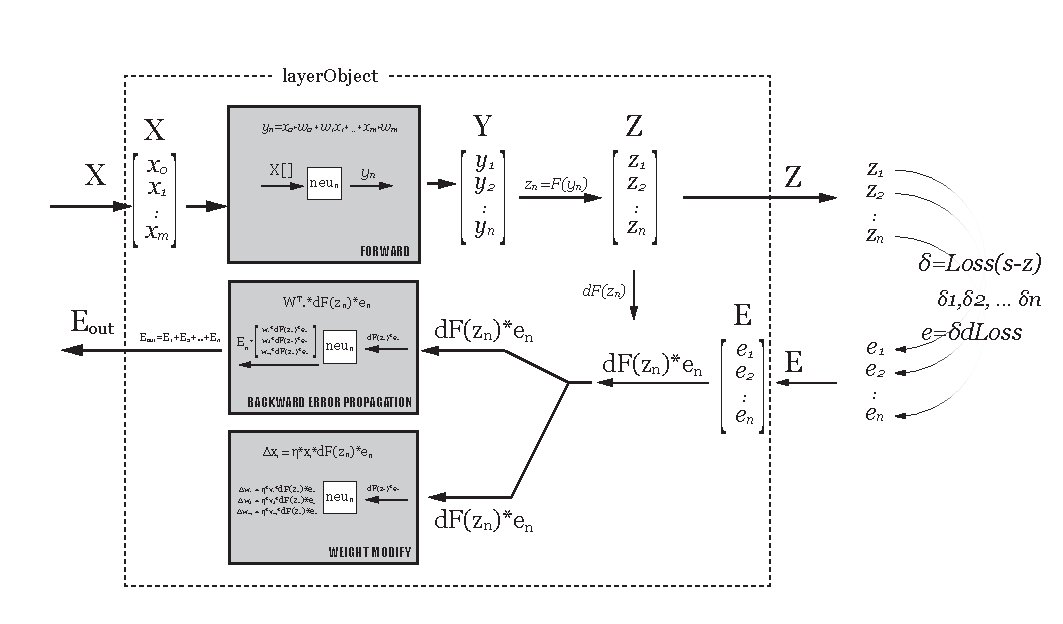
\includegraphics[width=0.74\linewidth]{rysunki/rys1_4.jpg} 
\end{figure} \newpage
Rozwiązanie w Javie oparto na własnej implementacji sieci MLP. Szczególny nacisk położono na czytelność kodu i idei kosztem wydajności. Wykorzystano wiedzę z poprzednich rozdziałów i napisano kod zgodnie z zasadami programowania obiektowego. Zasady hermetyzacji wymuszają utworzenie dwu współpracujących ze sobą obiektów: neurosumatora oraz warstwy. Własnością warstwy jest rodzaj funkcji aktywacji, a jej metodą jest obliczenie pochodnej funkcji aktywacji w punkcie pracy.
%%
%%
\begin{figure}[ht]
    	\centering 
            \includegraphics[width=0.72\linewidth]{rysunki/zad2.jpg} 
            \caption{Zadanie 2 - zestawienie czasów uczenia perceptronu MLP }
\end{figure} 
%%
\begin{figure}[ht]
    	\centering 
            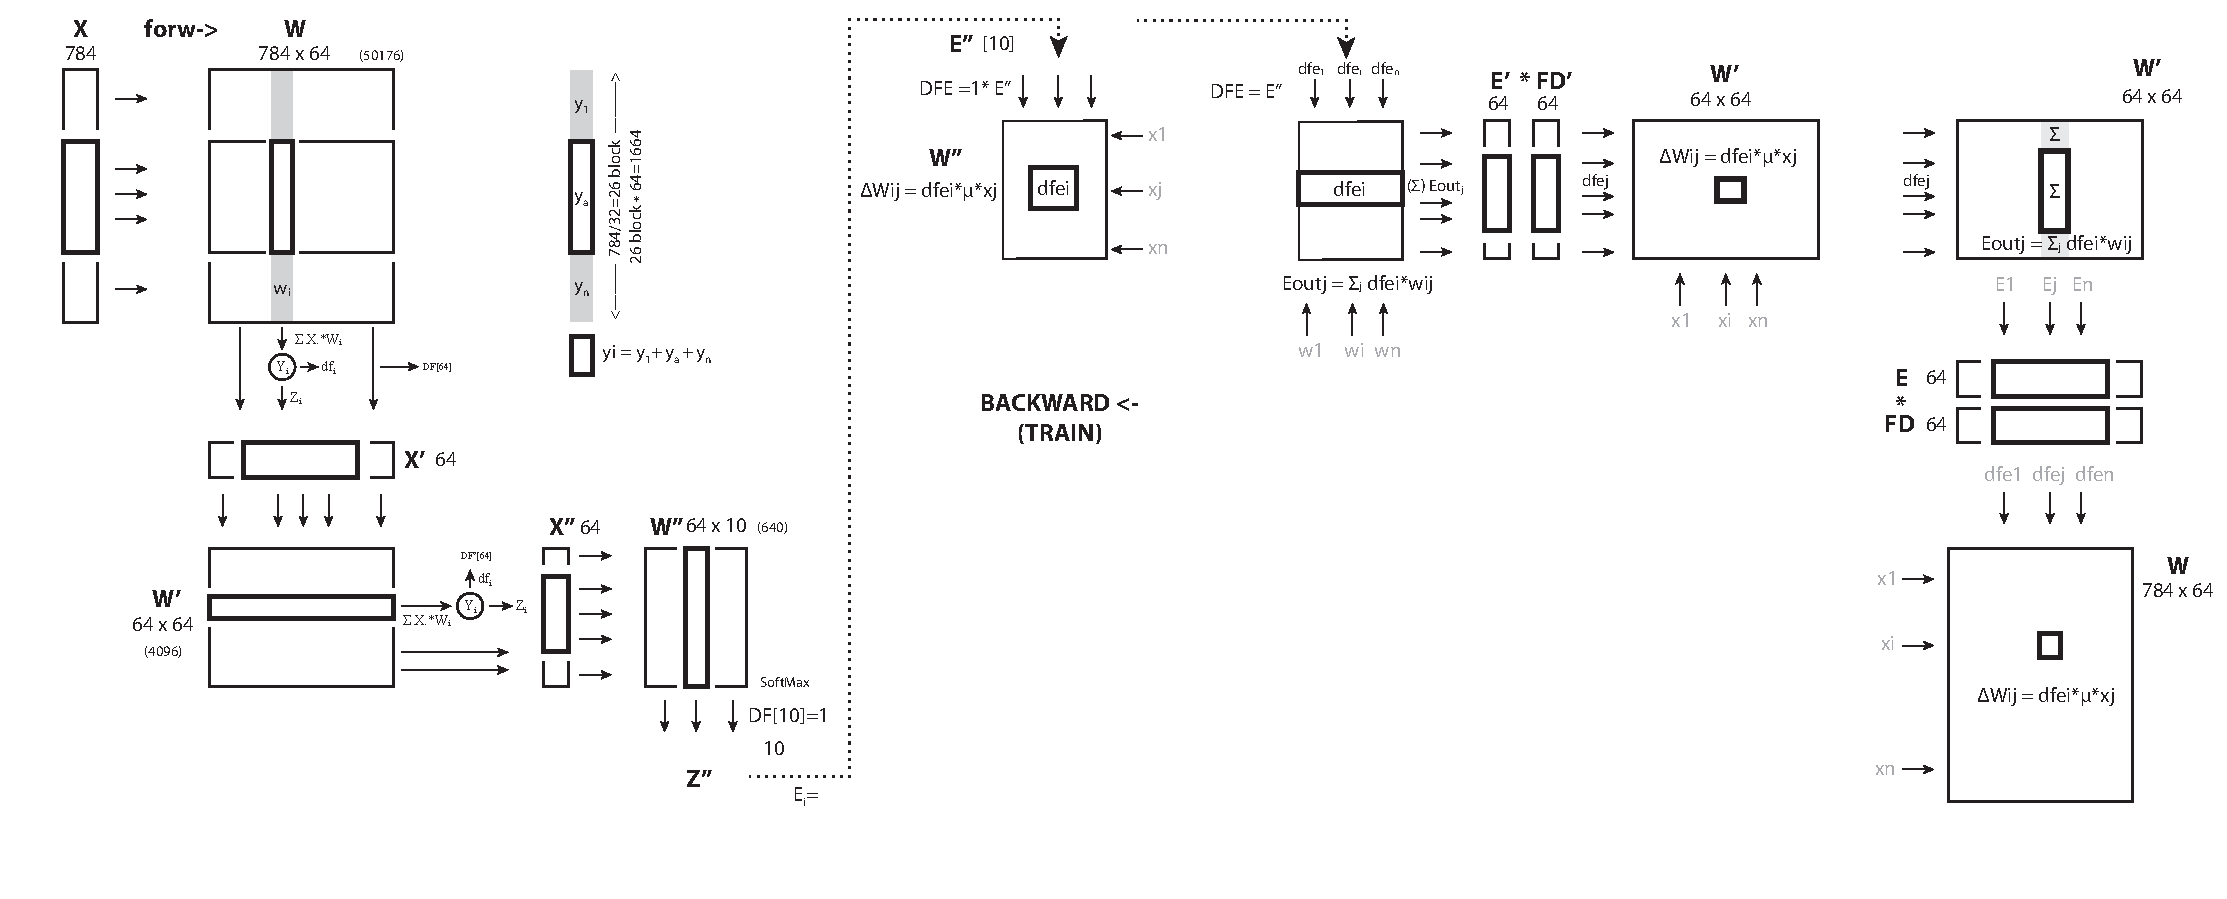
\includegraphics[width=0.72\linewidth]{rysunki/CUDA_train_process.jpg} 
            \caption{Zadanie 2 - obliczenia na GPU}
\end{figure}
%%
\begin{figure}[ht]
    	\centering 
            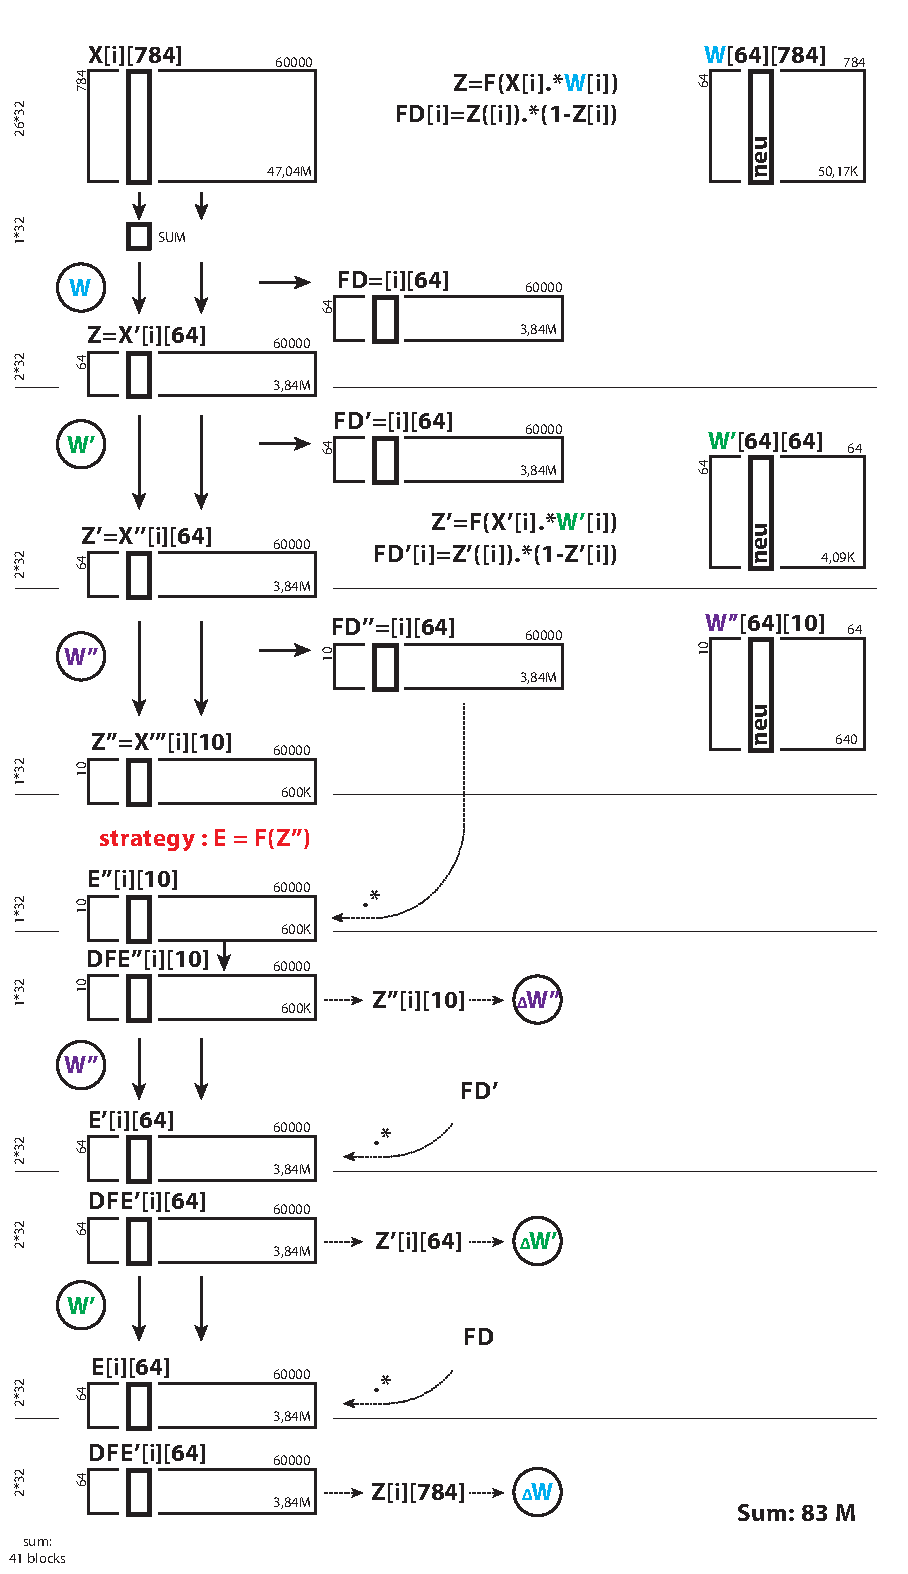
\includegraphics[width=0.42\linewidth]{rysunki/CUDA_memory.jpg} 
            \caption{Zadanie 2 - obliczenia na GPU mapa pamięci}
\end{figure}
%%
\section{ Zadanie 3 - sieć splotowa }
Zadanie polegało na zbudowaniu modelu sieci splotowej CNN połączonej z siecią MLP, wg. struktury LaNet-5 zaproponowanej przez prof. Yann LeCun \cite{YannCnn}  przedstawionej m.in. w \cite{Osowski2023}.
%%
%%
Przeprowadzeniu procesu uczenia sieci, polegającego na rozpoznawaniu cyfr pisanych ręcznie. Założono wykonanie 100 epok uczenia, przy wykorzystaniu 100\% objętości zbioru danych uczących.
%%
Struktura sieci:
\begin{itemize}
    \item Warstwa 1: Wejście obraz 28x28 pikseli 1 kanał.
    \item Warstwa 2: Konwolucyjna, 20 @ filtr 5x5, aktywacja ReLU.
    \item Warstwa 3: Normalizacja
    \item Warstwa 4: PoolMax, rozmiar 2x2, krok 2x2
    \item Warstwa 5: Spłaszczenie obrazu do jednowymiarowej tablicy
    \item Warstwa 6: MLP: 64 neurony, aktywacja ReLU
    \item Warstwa 7: MLP: 10 neuronów, wyjście Softmax
\end{itemize} 
%%
%%
\begin{center}
%%
\begin{tabular}{ |c|c| }  \hline
 Python PyTorch & Python Tensorflow.Keras \\
 \hline
    \begin{lstlisting}[language=c++,numbers=none,basicstyle=\tiny ,frame=none]
\\ CITE -> https://www.datacamp.com/
\\       tutorial/pytorch-cnn-tutorial
\\ Javier Canales Luna

class CNN(nn.Module):
def __init__(self, in_channels, num_classes):
    super(CNN, self).__init__()
    self.conv1 = nn.Conv2d(in_channels=in_channels, \
    out_channels=20, kernel_size=5, padding=1)
    self.norm  = nn.BatchNorm2d(20)
    self.pool = nn.MaxPool2d(kernel_size=2, stride=2)
    self.fc1 = nn.Linear( 3380, 64 )
    self.fc2 = nn.Linear( 64, num_classes )

def forward(self, x):
    x = F.relu(self.conv1(x))
    x = self.norm(x)
    x = self.pool(x)
    x = x.reshape(x.shape[0], -1)
    x = self.fc1(x)
    x = self.fc2(x)
    return x

start=time.time()
for epoch in range(epochs):
   scores = model(data)
   loss = criterion(scores, targets)
   optimizer.zero_grad()
   loss.backward()
   optimizer.step()
    \end{lstlisting}
    
 & 

\begin{lstlisting}[language=c++,numbers=none,basicstyle=\tiny ,frame=none]
\\ CITE -> https://keras.io/examples/
\\              vision/mnist_convnet/

 def AlexNet():
   NUMBER_OF_CLASSES = 10
   return keras.models.Sequential([
      keras.layers.Input(shape=( 28, 28, 1 )),
      keras.layers.Conv2D(name='conv1', \
      filters=20, kernel_size=(5,5), \
      activation='relu' ),
      keras.layers.BatchNormalization(),
      keras.layers.MaxPool2D(pool_size=(2,2), \
      strides=(2,2)),
      keras.layers.Flatten(),
      keras.layers.Dense(64, activation='relu'),
      keras.layers.Dense(10, activation='softmax')
])
model = AlexNet()
model.compile(optimizer='adam',
  loss='sparse_categorical_crossentropy',
  metrics=['accuracy'])
start=time.time()

with tf.device('/device:GPU:0'):
   model.fit(trainX, trainY, epochs=epochs, verbose=0)

    \end{lstlisting}
 
 \\

 \hline 
\end{tabular}
\end{center}
\newpage
W zadaniu wykorzystano dane z zadania 2, Dwa rozwiązania zostały napisane w Pythonie z wykorzystaniem bibliotek PyTorch oraz Tensorflow. Jedno rozwiązanie powstało w Matlabie z wykorzystaniem bibliotek systemowych. W języku Java napisano własne rozwiązanie, w którym przyjęto te same założenia i strukturę jak w zadaniu 2, rozszerzono działanie klas w projekcie tak by realizowały sieć splotową CNN oraz działanie warstw pomocniczych, ReLU, Flatten, Max i Avg.
%%
\begin{figure}[ht]
    	\centering 
            \includegraphics[width=0.72\linewidth]{rysunki/zad3.jpg} 
            \caption{Zadanie 3 - zestawienie czasów uczenia sieci CNN }
\end{figure} \newpage














\newpage
\section{ Zadanie 4 - głęboka sieć splotowa }
Zadanie polegało na zbudowaniu modelu głębokiej sieci splotowej CNN i nauczeniu sieci rozpoznawania twarzy. Przygotowany zbiór zdjęć uczących i testowych pochodził z zasobów publicznych internetu. 
~ \newline
\begin{figure}[ht]
    	\centering 
            \includegraphics[width=0.8\linewidth]{rysunki/zad4.jpg} 
            \caption{ Zadanie 4 - zestawienie czasów uczenia sieci głębokiej CNN }
\end{figure} 
~ \newline
\begin{figure}[ht]
    	\centering 
            \includegraphics[width=0.95\linewidth]{rysunki/zad4.jpg} 
\end{figure} 
\newline 
Rozwiązanie zrealizowano w dwu językach: Matlab i Python Tensorflow. 







\section{ Zadanie 5 - widzenie komputerowe }
Zadanie polegało na zbudowaniu aplikacji Yolo8 w językach Python i C++, z wykorzystaniem nauczonego modelu dostarczonych przez ultralytics. Oceniono czas wykonania rozpoznawania obiektów na obrazie. Porównania dokonano tak jak w poprzednich przypadkach w środowisku wyposażonym w kartę graficzną, a następnie powtórzono w tym samym środowisku już bez karty.

~ \newline
\begin{figure}[ht]
    	\centering 
            \includegraphics[width=0.8\linewidth]{rysunki/zad5.jpg} 
            \caption{ Zadanie 4 - zestawienie czasów rozpoznawania obiektów Yolo8 }
\end{figure} 

    %\chapter{Podsumowanie wyników i porównanie języków}
    %
% W tym rozdziale opisane będą aspekty języków, przedstawiono informacje o wykorzystanych

% bibliotekach, pokazano fragmenty kodu.


\section{ Aspekty języków }

\subsection{ Popularność języka }
Duża popularność języka zapewnia łatwy dostęp do dużej społeczności osób pracujących nad jego rozwojem. Dla dynamicznie rozwijających się języków powstaje wiele bibliotek, środowisk IDE, narzędzi, a także literatury i przykładów ich zastosowania w rozwiązywaniu konkretnych zadań. Do zastosowania w projektowanych rozwiązaniach warto wybierać języki popularne i nowoczesne, aby uniknąć trudności ze znalezieniem specjalistów do pracy nad projektem. 

\subsection{ Dostępność bibliotek }
Dla otwartych języków programowania powstaje wiele narzędzi i bibliotek, z których duża część jest udostępniana społeczności na różne sposoby. Dla rozwiązań komercyjnych bibliotek jest mniej, natomiast ich jakość najczęściej jest bardzo wysoka, dokumentacja dopracowana a pomoc techniczna łatwo dostępna. 

\subsection{ Wygoda instalacji }
Instalacja języka wraz ze środowiskiem może różnić się znacznie w zależności od systemu operacyjnego. Języki niższych poziomów integrujące się bardziej z systemem operacyjnym mogą być trudniejsze w instalacji i konfiguracji do pracy z np. kartami graficznymi. 

\subsection{ Stopień wykorzystania GPU }
W modelowaniu sieci głębokich wykorzystanie potencjału kart graficznych ma znaczenie kluczowe dla realizacji wydajnych modeli. 

\subsection{ Koszt licencji }
Większość języków i środowisk jest dostępna na licencji otwartej. Wykorzystanie niektórych języków, bibliotek czy środowisk IDE wiąże się z koniecznością zakupu licencji. Wykorzystanie w celach komercyjnych może wymagać zakupu innej, droższej licencji niż wykorzystanie w celach naukowych. 

\subsection{ Wygoda użytkowania }
W większości języków programowania ogólnego przeznaczenia stosuje się bardzo podobne konstrukcje i pracuje się na podobnych rodzajach danych. Języki programowania wysokiego poziomu bazują na bytach abstrakcyjnych, tworzenie kodu jest łatwe i nie wymaga od programisty znajomości dokładnej budowy komputera, znajomości sposobu działania pamięci czy rodzaju procesora na którym będzie uruchamiany program. Nauka programowania w językach wysokiego poziomu jest dużo szybsza niż w językach niższego poziomu jak np. C++, w którym mamy do czynienia ze ścisłą kontrolą typów przy jednoczesnym występowaniu wskaźników, referencji i ramek stosu, czy też w Asemblerze, do programowania w którym niezbędna jest wiedza nie tylko z zakresu np. sposobów reprezentacji liczb w pamięci, przeliczaniu z systemów szesnastkowych na dziesiętne, ale także z zakresu pracy na rejestrach, stosie, wywołaniach przerwań systemowych czy odwołań do funkcji systemu operacyjnego.  \newpage

\section{Python}

\begin{figure}[h]
    	\centering 
            \includegraphics[width=0.9\linewidth]{rysunki/LANG_python.jpg} 
            \caption{Zestawienie aspektów języków }
\end{figure} 
Według bulldogjob.pl najpopularniejszym językiem programowania jest Python \cite{popularnoscJezykow}. Jest to język młody, jednak prężnie rozwijany i bardzo modny. Składa się na to kilka przyczyn. Po pierwsze - jest to język darmowy  (z wyjątkiem specjalistycznych bibliotek). Po drugie - ma bardzo niski próg wejścia. Aby pisać kod w Pythonie, nie trzeba posiadać specjalistycznej wiedzy technicznej ani szczegółowo znać budowy komputera. Naukę programowania w tym języku rozpoczynają już dzieci w wieku szkolnym. Pisanie kodu jest bardzo przyjemne, w kontrolowaniu typów zmiennych pomagają biblioteki narzędziowe. Społeczność użytkowników jest bardzo pomocna, a w sieci znajdziemy dużo przykładów, samouczków i dokumentacji. Istnieje dużo bibliotek, także bibliotek do tworzenia modeli sieci neuronowych. 
Dla poznawania, trenowania modeli AI nadaje się idealnie.
Niestety instalacja systemu z obsługą najnowocześniejszych kart graficznych może być kłopotliwa.


\subsection{Conda, Anaconda, wirtualne środowiska}
Istnieje wiele rozwiązań pomagających zainstalować środowisko, a także budować wiele wirtualnych środowisk na jednej maszynie.

\subsection{Tensorflow}
Biblioteka Tensorflow wymaga rekompilacji do współpracy z GPU. Wersja instalowana z pakietów współpracuje z CPU i wykorzystuje rozkazy procesora AVX. Sprawia trudności przy instalacji, 

\subsection{Scikit-learn}

\subsection{PyTorch}
Wygodna do zainstalowania, bardzo współpracuje bardzo dobrze z procesorami graficznymi zarówno od NVidia, ale także może wykorzystać karty AMD. 







\section{Matlab}
Środowisko Matlab nie jest ujęte w zestawieniu bulldogjob.pl \cite{popularnoscJezykow}. Jest to środowisko płatne, tworzone i wykorzystywane przez środowiska akademickie. Jest przykładem wzorowej obsługi procesu instalacji oprogramowania i wsparcia obsługi kart graficznych. Pisanie kodu jest wygodne, a dostarczona dokumentacja i przykłady są obszerne i wygodne w użyciu. Jedynym, co może być mylące jest rozpoczynanie indeksów od 1. \newline
Dodatek Parallel computing w Matlab umożliwia wykonywanie obliczeń równolegle, w osobnych wątkach, procesach, a także z wykorzystaniem kart graficznych (obecnie tylko NVidia). Dodatki Optimalization Toolbox i Optimalization Computing Toolbox optymalizują tworzony kod, dzięki czemu zwiększają jego wydajność. Dodatek Deep Learning Toolbox dostarcza gotowych metod do obliczeń sieci neuronowych.

\section{C++}
Język C/C++ wg. bulldogjob.pl osiąga popularność na poziomie 6.6\% \cite{popularnoscJezykow}. C++ jest językiem, który nieco traci popularność na korzyść np. Pythona czy Rust. Jest to język darmowy, a integracja ze sterownikami i bibliotekami kart graficznych jest natywna. Idealnie pracuje w systemach Linux, ale dobrze działa także w Windows z Microsoft Visual Studio.
Jest to język kompilowany, w którym budowanie programu trwa dłużej niż w Pythonie czy Matlabie, jednak skompilowana aplikacja działa bardzo szybko. Język ten dobrze obsługuje karty graficzne. Jednak stawia duże wymagania użytkownikowi piszącemu kod. Do dobrego wykorzystania potencjału wymaga rozumienia procesów zachodzących w sprzęcie, znajomości wielu pojęć języka oraz dobrego poruszania się w typach danych. 

\section{Java}
Według bulldogjob.pl wskaźnik popularności dla języka Java wynosi 26.2\% \cite{popularnoscJezykow}. Java jest językiem podobnym do C++, jest to język kompilowany do kodu bajtowego uruchamianego w maszynie wirtualnej. Ma ścisłą kontrolę typów. Niektóre wersje wymagają opłacenia licencji, większość jednak jest darmowa. Wykonywalny kod działa dość szybko, nieco wolniej niż C++. Instalacja wymaga nieco uwagi. Istnieją biblioteki umożliwiające wsparcie obliczeń na kartach graficznych, jednak w tej pracy nie wykorzystywano tych bibliotek. Jest rzadko wykorzystywany do modelowania sieci neuronowych. 
~ \newpage


\section {Podsumowanie i wnioski}
\begin{figure}[h]
    	\centering 
            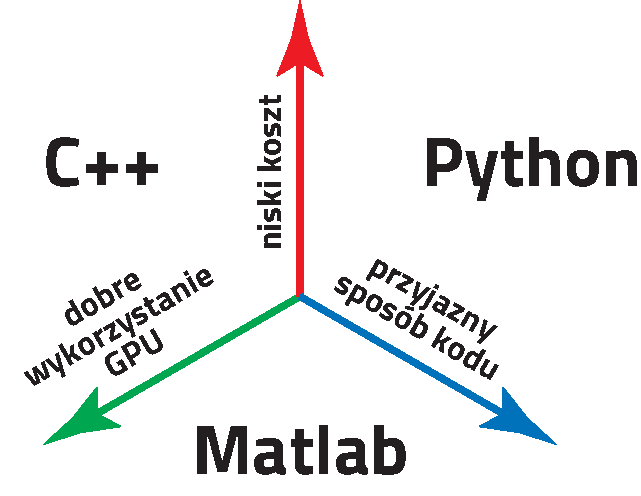
\includegraphics[width=0.5\linewidth]{rysunki/lang.jpg} 
            \caption{ Priorytety przy wyborze języka }
\end{figure} 
Przy wyborze języka trzeba zdecydować się na dwa z trzech priorytetów, jeden niestety trzeba odrzucić. Najwydajniejsze języki to C++ i Matlab. Najwygodniej pracuje się w Pythonie więc jest najczęściej wybierany do tworzenia modeli w celach  badawczych. Duże produkcyjne modele powstają zwykle w języku C/C++ i są uruchamiane w środowiskach serwerowych. 

\section{Dodatkowe wnioski}

\subsection{Zadanie 3}
Zbliżone czasy wykonania zadania 3 dla PyTorch z użyciem GPU i bez - sugerują, że możliwości GPU nie zostały użyte prawidłowo.

Poprawa kodu powoduje zdecydowane skrócenie czasu wykonania, jednocześnie zmienia wnioski wynikające z zestawienia: 

\begin{lstlisting}
-------------
CUDA available. Using GPU acceleration.
cuda
(59400, 1, 28, 28)
tensor([13.2702, -8.9589,  2.4638,  0.5280, -4.6336,  
  2.0661,  0.6992,  0.2631, 0.6639,  0.2546], 
  device='cuda:0', grad_fn=<SelectBackward0>)
  
# Python PyTorch 2.0 60000 Images, 100 Epoch 
  Time:  29.587559938430786
  Test accuracy: 0.6212121248245239
------------------
\end{lstlisting}

\chapter{uwagi}

Komentarze do pracy
2 Wydajność - wydajność czego?
2.1 Nie rozumiem po co wspominać o tym i to zaledwie w 2 zdaniach? (Maszyna Turinga)
2.2 Czy chodzi wyłącznie o translację punktów czy raczej o coś więcej (macierze na to wskazują). Nie wiem jak rozpisany wzór ma się do tych macierzy. 
Ogólnie rozdział 2 jest niezrozumiały. Wydaje mi się, że dostrzegam ideę, czyli pokazanie sposobów realizacji podstawowych obliczeń dodawania i mnożenia (których to operacji w wielu dziedzinach trzeba wykonywać miliardy czy biliony na sekundę), ale to co jest napisane jest niezrozumiałe, powyrywane z kontekstu, fragmentaryczne. Raczej trzeba wyjść od zdefiniowania tej potrzeby i potem pokazać, jak to w kolejnych etapach rozwoju komputerów robiono. ()
 
3 (Model perceptronu warstwowego MLP)
Nie można zaczynać rozdziału od rysunku.
Perceptron jest WIELOwarstwowy
W ogóle nie wiadomo po co o tym jest napisane. To jakoś trzeba uzasadnić.
 
4 (Modele sieci splotowych CNN)
Też nie wiadomo dlaczego nagle o tego rodzaju sieci Pan wspomina. We wszystkich tych rozdziałach brakuje jakiegoś wprowadzenia, które uzasadniłoby pisanie o tym. Plus te 3 rozdziały należy wrzucić do jednego, bo to raptem 11 stron jest, w tym sporo rysunków.
 
5.1
Kod w Javie opisany jako Python. Brakuje kodu własnej implementacji w Pythonie i Matlabie, nie wiadomo co to JavaBigDecimal. na wykresie jest C, a nie C++. Choć ten kod to w sumie C, a nie C++. DLa C++ powszechnie używana jest biblioteka Eigen, w której jest m.in. regresja liniowa. Skoro sprawdza Pan funkcję "wbudowaną" dla Pythona, to wypadałoby sprawdzić analogiczną dla C++.
 
5.2
Znowu niejasności i nie wiadomo dlaczego tak, a nie inaczej, oraz jak. Są 2 fragmenty kodu, ale sprawdzanych wersji kodu było znacznie więcej. Nie wiadomo więc co i jak tam było zrobione. W szczególności nie wiadomo jak uruchomił Pan sci-kit na GPU. Normalnie nie bardzo się da chyba.
Ogólnie eksperyment pokazuje, że nie warto angażować GPU do relatywnie prostych sieci i małych zbiorów danych. 
 
5.3, 5.4 Ogólnie pokazują, że dla większych sieci GPU się opłaca
5.5 nie rozumiem podpisu C++ Torch? Yolo8 w pythonie działa tak samo szybko na CPU i GPU? Coś tu nie gra. Sprawdziłem i jest kilkukrotna (zależy od sieci)
 
 
Na razie praca, w bardzo chaotyczny i niejasny sposób, pokazuje (i to nie zawsze), że GPU opłaca się dla większych sieci, a dla mniejszych nie. Zasadnicze pytanie: w jakim języku najlepiej napisać kod dla głębokich sieci neuronowych pozostaje bez odpowiedzi. Za mało jest tu eksperymentów i są one praktycznie nieopisane. O rozpoznawaniu twarzy są 2 zdania! A powinno być 10 stron. W założeniach miało to być zrobione w Matlabie, w Pythonie i jeszcze w czymś.  W zakresie ZABRAKŁO wyszczególnienia pytorcha, jako że torch i tensorflow to dwie podstawowe biblioteki do głębokiego uczenia. Tu brakuje też rozróżnienia czasu uczenia i czasu wnioskowania. Podejrzany jest też fakt, że Matlab jest szybszy. No ale kompletnie nie wiadomo co tam było robione i jak. I tak wygląda cała praca... To MUSI zostać skonkretyzowane. Trzeba pokazać cały proces w Matlabie, w Pythonie (najlepiej z tensorflow i z pytorchem) oraz ewentualnie jeszcze w torchc++ (o ile da się to łatwo uruchomić). Czyli potrzebny jest kod, przebieg uczenia, czas uczenia, czas wnioskowania, porównanie dokładności sieci, potem ocena łatwości przeprowadzenia całego procesu - w jakim środowisku jest to najprostsze, najprzyjaźniejsze, w jakim mamy większą kontrolę nad tym co robimy. I tak dla kilku zadań wymienionych w zakresie pracy. Wówczas będzie można porównać te języki
 

\chapter{test}
"Sztuczna inteligencja" zyskała w ostatnim czasie ogromną popularność. Wielkie firmy technologiczne udostępniły użytkownikom możliwość komunikacji ze swoimi wielkimi modelami językowymi LLM. Powstały modele językowe pracujące w języku polskim, m.in "Bielik", na dziś dostępna jest wersja BIELIK-11B-v2 mająca 11 000 000 parametrów. Uczenie tak dużych modeli szybciej niż konkurencja wymaga posiadania wielkich centrów obliczeniowych. 


W cieniu modeli językowych pozostają inne, dużo mniej medialne rozwiązania wykorzystywane od dziesięcioleci w przemyśle modele sieci MLP \cite{Korbicz1994},  Dziedzina "widzenia komputerowego" dostarcza modeli sieci głębokich CNN używanych w rozpoznawaniu obrazów, ich klasyfikacji a także  orientacji w przestrzeni. Modele te są używane zwłaszcza w robotyce. 
\cite{Osowski2023},
 \cite{Osowski2020}.
 \cite{rasheed},

 \cite{conv},
\cite{conv1}.

% ***********************

    % Bibliografia - musi być, jest w pliku EE-dyplom.bib
    % Bibliography - must exist, is in the file EE-dyplom.bib
    \bibliografia

    % Strony końcowe - można zakomentować, jeśli zbędne
    % Additional pages - comment out if not needed
    
    % Wykaz symboli i skrótów - patrz opis w tekście przykładowym
    \acronymslist
    % Spis rysunków
    \listoffigures
    % Spis tabel
    \listoftables
    % Załączniki (plik appendices.tex)
    \easyappendices
  

\end{document}
%%%%%%%%%%%%%%%%%%%%%%%%%%%%%%%%%%%%%%%%%%%%%%%%%%%%%%%%%%%%%%%%%%%%%%%%%%%